% Tento soubor nahraďte vlastním souborem s obsahem práce.
%=========================================================================
% Autoři: Michal Bidlo, Bohuslav Křena, Jaroslav Dytrych, Petr Veigend a Adam Herout 2019

% Pro kompilaci po částech (viz projekt.tex), nutno odkomentovat a upravit
%\documentclass[../projekt.tex]{subfiles}
%\begin{document}

\chapter{Úvod}
Balancující robot je specifický druh mobilního robota, který se bez vnějšího zásahu dokáže udržet v přirozeně nestabilní vzpřímené poloze. Na rozdíl od vícekolových robotů vyniká vysokou obratností, méně složitou konstrukcí a lepší prostupností ve stísněných prostorech. Dále je takový robot vynikajícím demonstrátorem různých ovládacích mechanismů.

K výběru tohoto tématu mě vedl zájem o robotiku, především o návrh a řízení systémů, které nejsou od přírody stabilní. Práce na dvoukolovém balancujícím robotovi mi umožnila propojit znalosti z oblasti mechatroniky, programování a elektroniky.

Tato práce se věnuje procesu tvorby takového robota -- od výběru komponent a stavby, až po naprogramování balančního mechanismu. Toto řešení je specifické využitím platformy Robot Operating System 2 (dále ROS2), která umožňuje vysokou modularitu a zároveň mnoho vestavěných nástrojů, které dále zjednodušují programování.

V teoretické části práce je vysvětleno fungování balancujícího robota a fyzikální princip obráceného kyvadla, na kterém je balancování založeno. Jsou zde také
ukázány již existující řešení. Kapitola \ref{chap4} popisuje konstrukci robota a vybrané komponenty. Zároveň je tu i výčet alternativních komponent a konstrukcí. V kapitole \ref{chap5} je vysvětleno použití platformy ROS2 a operačního systému Ubuntu s jádrem operačního systému operujícím v reálném čase. Obsahuje také vlastní implementaci balančního mechanismu za použití PID regulátorů, čtení úhlu náklonu, rychlosti otáčení motorů a sledování okolního prostředí. Testování a výsledky jsou v kapitole \ref{chap6}.
\chapter{Přehled problematiky}
\label{chap2}
V této kapitole jsou probrány teoretické základy potřebné k pochopení způsobu vyvažování dvoukolového robota. Je zde také výčet již existujících řešení (jak z akademické, tak z~komerční sféry) a popis technologií, které využívají.

\section{Vyvažovací mechanismus}
Balancování dvoukolových robotů je založené na fyzikálním principu obráceného kyvadla, který je podrobně vysvětlen v následující kapitole. Fungování robota je svým způsobem podobné principu, jakým udržuje rovnováhu lidské tělo – to je totiž ve vzpřímené poloze také přirozeně nestabilní a vyžaduje neustálé zásahy k udržení této polohy. A zatímco člověk vnímá svůj náklon pomocí systému vnitřního ucha a balancování provádí přesným pohybem mnoha různých svalů po těle, dvoukolový robot vnímá úhel náklonu pomocí přesných senzorů (gyroskop a akcelerometr) a balancování zajišťuje přesně vypočítaným pohybem kol vpřed a vzad. 

Jízda robota je zajištěna změnou cílového náklonu. Zatímco pro stání na místě je obecně cílový úhel 0 stupňů, posunem tohoto cílového úhlu se změní chování regulátoru, který pro udržení rovnováhy zvolí pohyb ve směru tohoto posunutého náklonu. Zatáčení se u dvoukolových robotů implementuje rozdílnou rychlostí otáčení kol.

\section{Inverzní kyvadlo}
Inverzní kyvadlo je klasickým problémem teorie řízení, kde skvěle znázorňuje výzvy balancování přirozeně nestabilních systémů. Inverzní kyvadlo má těžiště nad pivotním bodem. Samotný pivotní bod se nachází na vozíku, který pohybem vpřed a vzad obstarává balancování. Bez těchto zásahů se kyvadlo vlivem gravitace vrací zpět do přirozeně stabilní polohy. 

Systém je znázorněn na obrázku \ref{kyvadlo}. Balancujeme kyvadlo o délce {\it l} a hmotnost {\it m}. {\it F} je síla, kterou posouváme pivotní bod.

Tento systém slouží jako zjednodušený model pro úlohy, jako je například balancující robot. Ten se sice na vozíku nenachází, ale otáčením kol pohybujeme se samotnou pivotní osou.

\begin{figure}
    \centering
    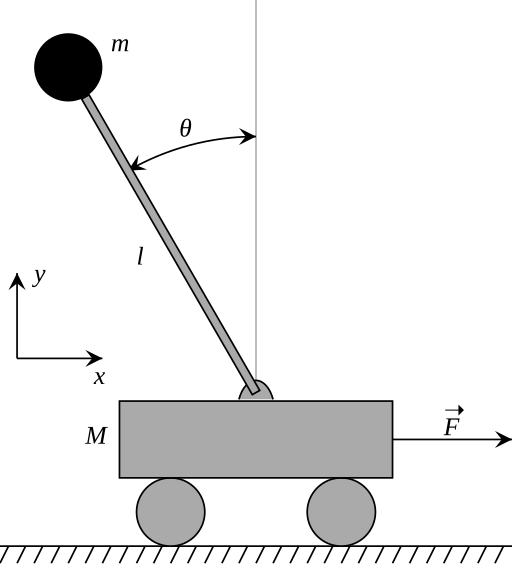
\includegraphics[width=0.5\linewidth]{obrazky-figures/512px-Cart-pendulum.svg.png}
    \caption{Model inverzního kyvadla na vozíku. Převzato z: \cite{kyvadlo_img}}
    \label{kyvadlo}
\end{figure}

Stabilizace obráceného kyvadla zahrnuje různé techniky řízení, včetně klasických PID regulátorů, lineárně kvadratických regulátorů (LQR) a pokročilejších metod, jako je modelové prediktivní řízení (MPC). Volba regulátoru významně ovlivňuje výkonnost systému, rezervu stability a odolnost vůči poruchám. \cite{kyvadlo}

\section{Metody vyvažování robota}
V robotice jsou chování a stabilita systému do značné míry určeny použitými metodami řízení. Tyto metody lze obecně rozdělit na řízení v otevřené a uzavřené smyčce (se zpětnou vazbou). V systému s otevřenou smyčkou se příkazy vydávají robotovi bez sledování výsledku -- takové přístupy jsou jednoduché, ale v nejistém nebo dynamickém prostředí nespolehlivé. Naproti tomu systémy s uzavřenou smyčkou využívají zpětnou vazbu od senzorů k úpravě činností v reálném čase, což umožňuje robustní výkonnost i v obtížných podmínkách. Většina moderních algoritmů řízení robotů, jako například PID a LQR pracuje v~rámci uzavřené smyčky.

\subsection*{PID}
PID regulátor je díky své jednoduchosti a účinnosti jednou z nejpoužívanějších řídicích strategií v robotice. Kombinuje tři členy: proporcionální (P), který reaguje na aktuální chybu, integrální (I), který kumuluje minulé chyby, a derivační (D), který předpovídá budoucí chyby na základě rychlosti změny. Výsledný řídicí signál u(t) se vypočítá jako:

\[
u(t) = r_0 e(t) + r_i \int_0^t e(\tau) \, d\tau + r_D \frac{de(t)}{dt}
\]

kde e(t) je chyba mezi požadovanou a skutečnou hodnotou a $r_0$, $r_i$, $r_D$ jsou příslušné zisky. PID je efektivní zejména pro lineární systémy a má nízké výpočetní nároky, takže je vhodný i pro platformy s omezenými zdroji, jako je Arduino nebo ESP32. \cite{PID}

\section{Existující řešení}
Tato podkapitola je věnována již existujícím řešením balancujících robotů. Jsou zde obsaženy jak školní projekty, tak komerční roboti. Popsáno je také použití různých typů komponent a regulátorů.

\subsection*{TUM Cascaded LQR Robot}
Autorem práce je Klaus Albert. K dosažení vysokého výkonu v reálném čase řídí robota mikrokontrolér AT32UC3C1512C. K pohybu využívá dva 6W kartáčové stejnosměrné motory vybavené přesným optickým enkodérem. Robot je vytisknut na 3D tiskárně a váží pouze 336 g (i s baterií). Jako regulátor využívá LQR.

Robot má dva režimy provozu. V prvním se chová jako standartní balancující robot. V~druhém módu využívá malé kolečko, které je připevněné v horní části konstrukce k jízdě ve vodorovném stavu. Oba režimy můžeme vidět na obrázku \ref{TUM_rob}. \cite{TUM_robot}

\begin{figure}[H]
  \centering
  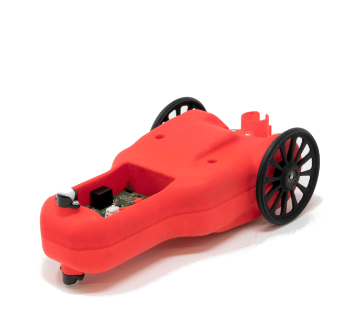
\includegraphics[width=0.5\linewidth]{obrazky-figures/leh_TUM.png}\hfill
  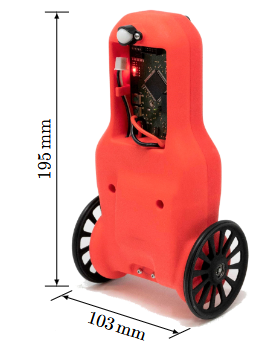
\includegraphics[width=0.5\linewidth]{obrazky-figures/stoj_TUM.png}
  \caption{TUM Cascaded LQR Robot, dostupné z \cite{TUM_robot}}
  \label{TUM_rob}
\end{figure}

\subsection*{Smart Two Wheels Balancing Robot}
Autorem práce je Hasan Alshahrani. Robot k provozu využívá dva různé mikrokontroléry -- ArduPilot Mega, což je deska určená k řízení různých dronů a RC letadel. Deska je přímo spojená s IMU modulem, ze kterého získává data o úhlu náklonu a úhlové rychlosti a Arduino Pro Mini, který obstarává čtení dat z enkodérů a pohyb motorů. Desky mezi sebou komunikují pomocí protokolu I²C. Jako regulátor je použito PID. Konstrukce je složená z~3D vytisknutých dílů a používá široká kola vhodná i do terénu -- viz obrázek \ref{SMART_bot}.

Díky využití mikrokontroléru určeného pro drony má robot zabudovaný kompas a GPS modul. Dokáže tedy následovat trasu podle zadaných navigačních bodů. \cite{smart}

\begin{figure}[H]
    \centering
    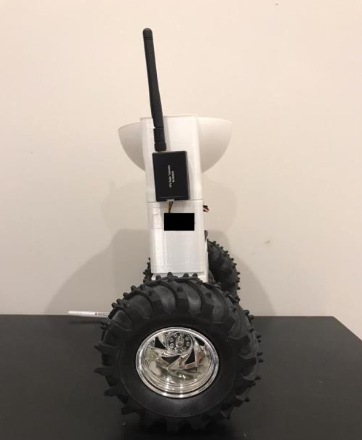
\includegraphics[width=0.6\linewidth]{obrazky-figures/smart_bot.png}
    \caption{Smart Two Wheels Balancing Robot, dostupné z: \cite{smart}}
    \label{SMART_bot}
\end{figure}

\subsection*{Handle}
Robota vytvořila americká firma Boston Dynamics. Má hmotnost 150~kg a měří 2 metry. Na rozdíl od ostatních robotů uvedených ve výčtu nemá pevné tělo -- je tvořený z několika částí spojených klouby, díky čemuž dokáže dynamicky měnit svoje těžiště. To mu umožňuje převážet břemeno o hmotnosti až 15~kg. Motory jsou elektrické, klouby jsou poháněny hydraulicky. Jedná se o skvělou ukázku výhod dvoukolových balancujících robotů -- díky malé základně se robot dokáže pohybovat i na místech, kde by vícekoloví roboti měli potíže. \cite{handle}

\begin{figure}[H]
    \centering
    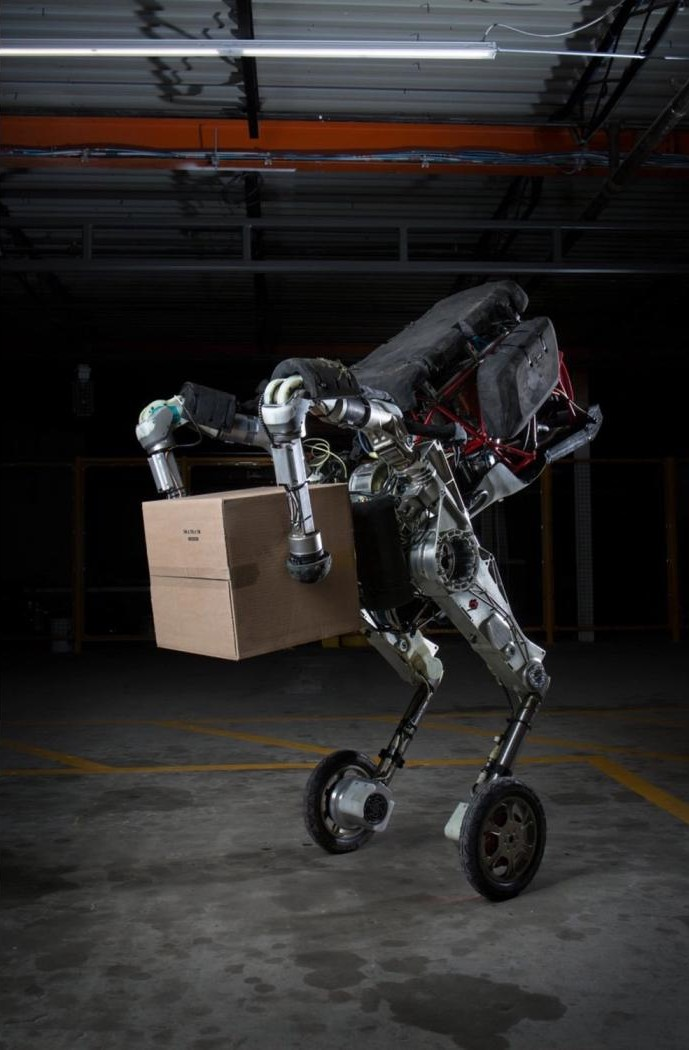
\includegraphics[width=0.6\linewidth]{obrazky-figures/handle.jpg}
    \caption{Handle, dostupné z: \cite{handle}}
    \label{handle}
\end{figure}

\chapter{Návrh vlastního řešení}
\label{chap3}
V této kapitole bude obecně popsáno, jaká řešení jsou zvolena pro jednotlivé problematiky balancujícího robota. Na konkrétní implementaci částí projektu bude odkazováno z textu.

\subsection*{Platforma}
Robot bude řízen platformou Raspberry Pi4B bez použití pomocných kontrolérů. To v praxi znamená, že veškeré senzory jako enkodéry motorů, či akcelerometr a gyroskop jsou připojeny přímo k Raspberry. Raspberry bude mít nainstalovaný operační systém s jádrem běžícím v reálném čase -- více o této problematice zde: \ref{system}. Samotný program balancujícího robota bude postavený v systému Robot operating system 2, který umožňuje celý projekt sestavit z jednotlivých modulů, které mezi sebou komunikují (a dokážou fungovat nezávisle na sobě).

Více o výběru platformy je v kapitole \ref{rsb}.

\subsection*{Vlastní konstrukce}
Konstrukce dvoukolového robota bude vytvořená na 3D tiskárně. Uvnitř bude baterie, která umožní provoz robota bez vnějšího zdroje energie a její nabíjení bude zajištěno pomocí USB-C. 

Robot bude mít dva stejnosměrné 12V kartáčové motory uložené v základně.

\subsection*{Balancování a pohyb}
Balancování bude zajišťovat dvojice PID regulátorů. První z nich z náklonu robota a úhlové rychlosti naklánění určí potřebnou sílu reakce motorů. Druhý regulátor z dat enkodérů zjistí, o kolik se robot vychýlil z počáteční pozice. Podle velikosti vychýlení vypočítá korekci, kterou následně pošle do prvního PID regulátoru.

Zatáčení robota bude obstarávat třetí PID regulátor. Ten sleduje rozdíl mezi pulzy z enkodérů a vypočítá chybu. Tím zajistí, že se robot nevychýlí ze směru kvůli nečekanému chování jednoho z motorů. Pokud bude potřeba s robotem zatočit, bude do tohoto PID regulátoru uměle vložená chyba mezi enkodéry, což povede ke korekci a zatočení. 

Více o implementaci balancování a zatáčení je v kapitole \ref{turn}.

\subsection*{Dálkové ovládání}
Robota bude možné dálkově ovládat z telefonu pomocí technologie Bluetooth. V aplikaci na mobilním telefonu bude přepínání mezi režimy pohybu robota a informace o stavu programu. Implementace dálkového ovládání je více probrána v kapitole \ref{remote}

\subsection*{Autonomní pohyb a manuální ovládání}
Robot bude mít dva režimy pohybu -- manuální a autonomní. V manuálním režimu bude směr jízdy a otáčení robota ovládán přímo z mobilního telefonu. V autonomním režimu bude robot využívat ultrazvukového měřiče vzdálenosti k jednoduchému pohybu s vyhýbáním se překážkám.

\chapter{Mechanická konstrukce a hardware} 
\label{chap4}
V kapitole jsou probrány varianty různých komponent potřebných pro funkci robota. U zvolených komponent je jejich popis a zdůvodnění jejich výběru. Na konci kapitoly je schéma zapojení, na které je odkazováno z jednotlivých podkapitol.

\section{Řídící platformy}
Výběr vhodného řídícího modulu zásadně ovlivňuje schopnosti celého systému. Mezi tři nejrozšířenější platformy patří Raspberry Pi, Arduino a ESP32, přičemž každá z nich má své silné stránky a omezení.

\subsection*{Raspberry Pi 4B}
\label{rsb}
Raspberry Pi 4B je jednodeskový počítač, který podporuje různé operační systémy založené na Linuxu, například Raspberry Pi OS a Ubuntu. Oproti Arduinu a ESP32 nabízí výrazně vyšší výpočetní výkon (čtyřjádrový procesor ARM Cortex-A72 s frekvencí 1.5~GHz). Deska má 4GB operační paměti, uložiště je obstaráno pomocí MicroSD karty. Má zabudovaný Wi-Fi a Bluetooth modul, nabízí několik USB a USB-C portů a také dva micro-HDMI konektory pro obrazový výstup. Napájení lze zajistit pomocí USB-C, nebo připojením regulovaného napětí v rozsahu 4.75~V -- 5.25~V. Při překročení napětí hrozí poškození desky, při příliš nízkém napětí deska nejprve omezí výkon, potom se sama vypne. Výrobce doporučuje alespoň 3A zdroj. Nevýhodou oproti ostatním deskám je vysoká cena. \cite{raspberry}

\subsection*{ESP32S}
Mikrokontrolér ESP32 nabízí dostatečnou výpočetní kapacitu, Wi-Fi a Bluetooth konektivitu a nízkou cenu. Má dvoujádrový procesor Xtensa LX7 s frekvencí až 240~MHz. Desku lze napájet pomocí USB-C, nebo připojením regulovaného napětí 3.3~V na 3.3~V pin. Deska má zabudovaný regulátor napětí, takže je ji také možno napájet připojením zdroje o napětí 5-10V na 5V pin. Díky nízké spotřebě a dostatečnému výkonu se jedná o častou volbu pro zařízení v internetu věcí (IoT). \cite{ESP32}

\subsection*{Arduino UNO R4}
Platformy Arduino jednoduché programovatelné open-source desky. Deska je zajímavá tím, že pro zajištění Wi-Fi a Bluetooth konektivity přímo obsahuje vestavěný ESP32S čip. Tato verze Arduina je poháněna jednojádrovým mikrokontrolérem Xtensa LX7 s frekvencí 48 MHz, jedná se tedy o nejméně výkonnou z těchto tří platforem. Velkou výhodou je možnost vstupního napájení 6~V až 24~V, což by jako jediné z desek umožnilo Arduinu v projektu fungovat bez regulátoru napětí. Nicméně kvůli nízkému výkonu není deska vhodná do projektů s větším rozsahem. \cite{arduino}

\subsection*{Zvolená varianta}
Jako řídící platforma byla zvolena deska Raspberry Pi4B ve verzi se 4 GB operační paměti. Poskytuje dostatečný výkon ke čtení a zpracování dat ze senzorů a jejich interpretaci na otáčky motoru. Jako jediná z desek umožňuje plnohodnotný operační systém, díky čemuž může projekt běžet ve frameworku Robot Operating system 2. 

Za operační systém byl zvolen Ubuntu server 22.04 LTS. Ten podporuje ROS2 v distribuci Humble Hawksbill, která měla v době začátku práce z používaných distribucí nejdelší projektovanou životnost a zároveň má vynikající dokumentaci.

Raspberry je na schématu zapojení znázorněno pod písmenem~H \ref{schema}.

\begin{figure}[H]
    \centering
    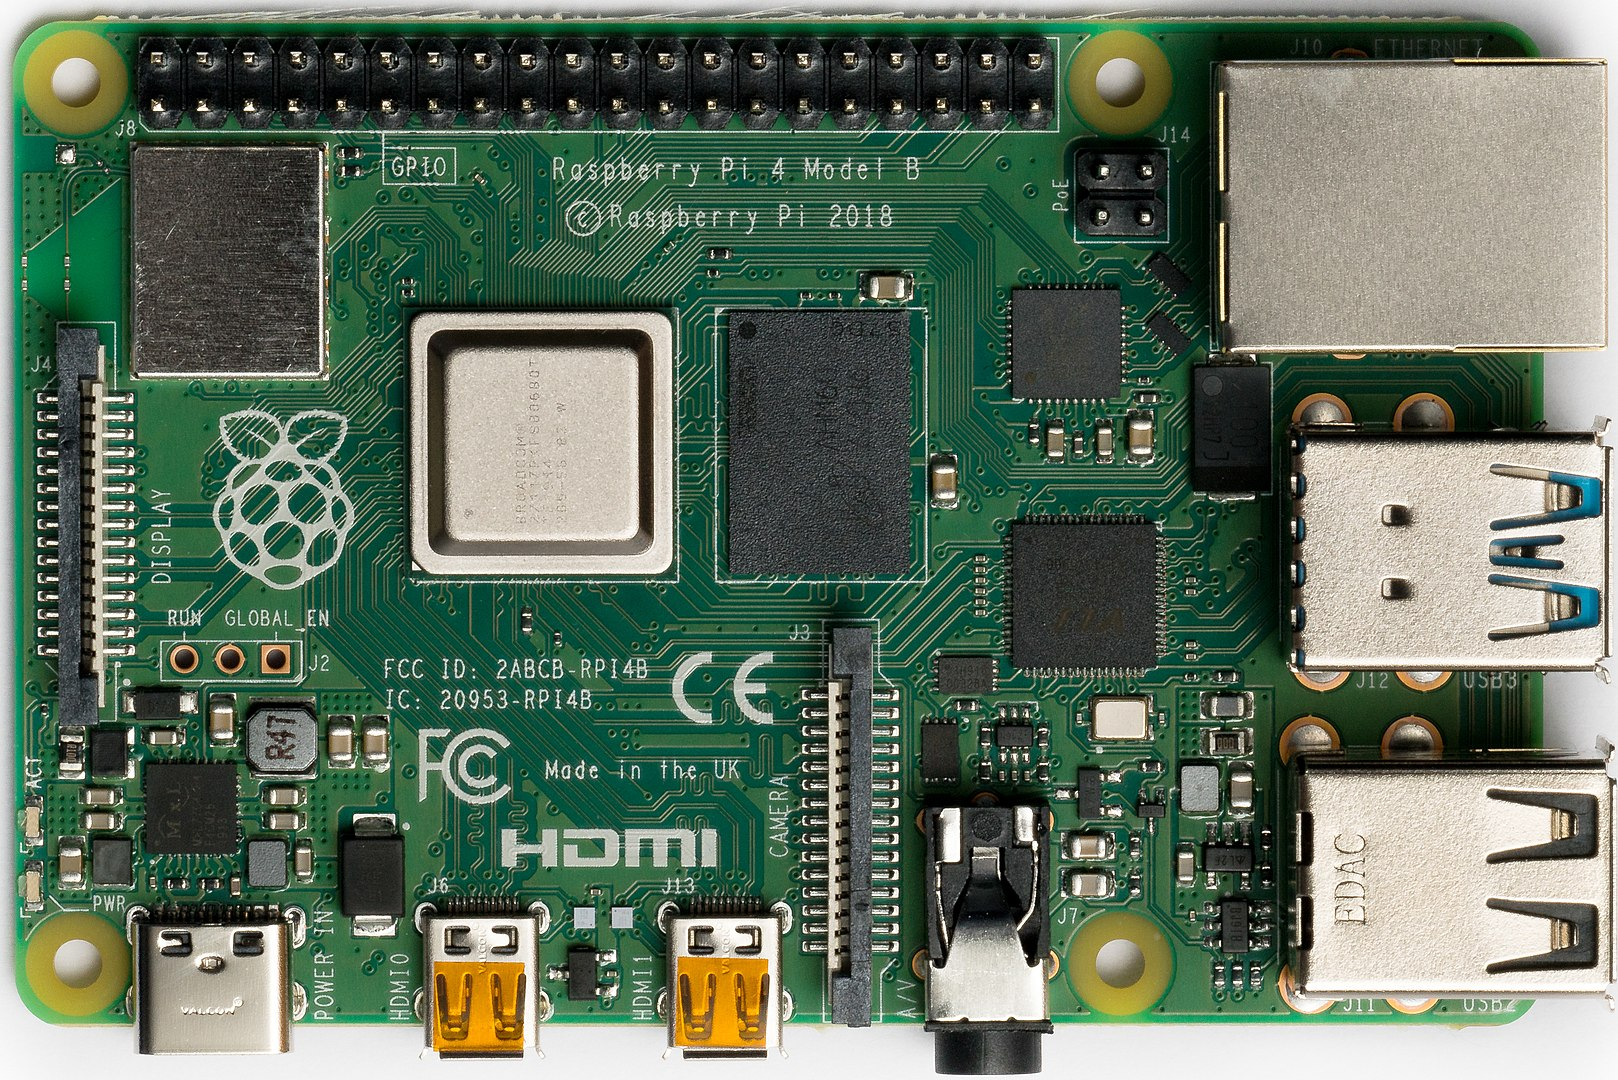
\includegraphics[width=0.5\linewidth]{obrazky-figures/raspberry.jpg}
    \caption{Raspberry Pi 4B, dostupné z: \cite{raspberry_img}}
    \label{raspberry}
\end{figure}

\section{Senzory}
\subsection*{Snímač náklonu}
Jako snímač náklonu byl zvolen modul GY-521 s čipem MPU6050. Má zabudovaný 3-osý gyroskop a 3-osý akcelerometr. Díky velmi dostupné ceně a dostatečné přesnosti je to jeden z nejčastějších modulů používaných v robotice. Velkou výhodou je, že obsahuje čip Digital Motion Processor, který dokáže sám interpretovat data z gyroskopu a akcelerometru a přes sběrnici I²C posílá už hotová data. Citlivost gyroskopu lze zvolit z hodnot: ±250  °/s, ±500  °/s, ±1000  °/s a ±2000  °/s a citlivost akcelerometru ±2g, ±4g, ±8g a ±16g \cite{IMU}. Nižší zvolená hodnota poskytuje vyšší přesnost měření, ale při rychlém pohybu se může saturovat a způsobit nepřesnost měření.

Kvůli absenci magnetometru trpí snímač na vznikající nepřesnost měření při delším běhu programu. Důležité je před spuštěním programu provést kalibraci modulu ve výchozí poloze.

Gyroskop a akcelerometr je na schématu zapojení znázorněn pod písmenem~I \ref{schema}.

\begin{figure}[H]
    \centering
    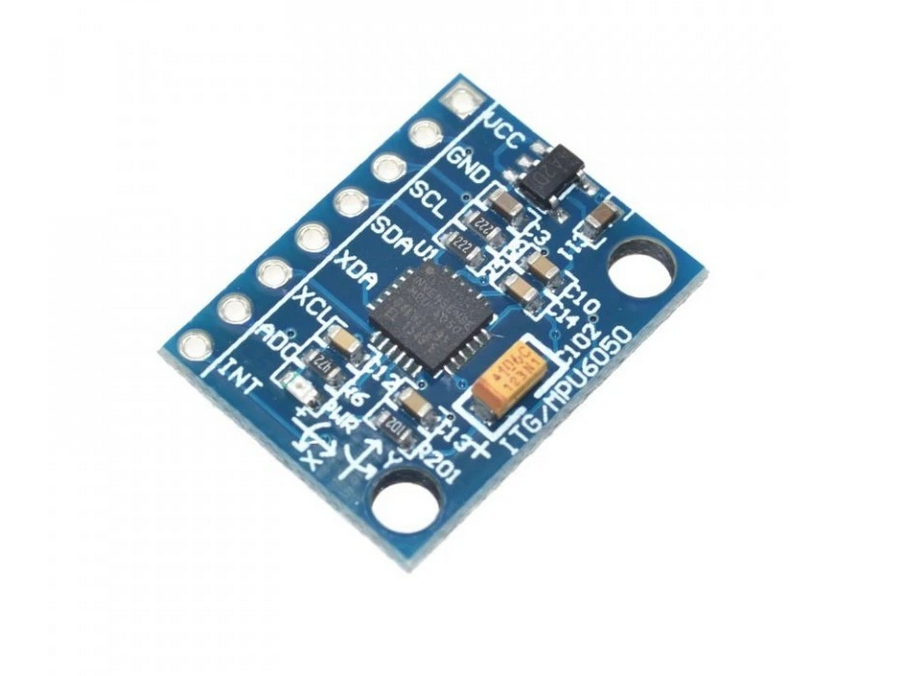
\includegraphics[width=0.5\linewidth]{obrazky-figures/IMU.png}
    \caption {GY-521, dostupné z: \cite{imu_img}}
    \label{raspberry}
\end{figure}

\subsection*{Ultrazvukový senzor}
\label{ultra_s}
Jedním z cílů práce je, aby byl robot schopen autonomního pohybu. Bylo tedy potřeba zvolit metodu, jak bude robot snímat své okolí. Existuje mnoho možností -- pokud například chceme, aby robot následoval vyznačenou čáru na zemi, můžeme zvolit kameru a z jejího výstupu určit nutné úpravy pohybu \cite{kamera}.

Pokročilým řešením je využití senzoru typu LIDAR. Ten pomocí laseru skenuje své okolí a poskytuje pro robota podrobný přehled, kde se nachází překážky. Toto řešení je ovšem finančně velmi náročné.

Pro projekt byl nakonec zvolen ultrazvukový měřič vzdálenosti HC-SR04. Tento typ senzoru funguje tak, že vyšle vysokofrekvenční zvuk (typicky nad 20 kHz -- pro člověka neslyšitelné) a změří, za jakou dobu se k němu vrátí odraz tohoto zvuku. V programu následně díky znalosti rychlosti zvuku ve vzduchu vypočítáme, jak je objekt daleko. HC-SR04 dokáže změřit předměty ve vzdálenosti 2 cm až 400 cm, což je pro potřeby projektu dostačující. Problémem řešení je, že při náklonu robota (který je potřebný k pohybu) může jako překážku registrovat i povrch, po kterém se robot pohybuje.

Podrobně je fungování senzoru znázorněno na obrázku \ref{ultra_s}. 

Ultrazvukový senzor je na schématu zapojení znázorněn pod písmenem~J \ref{schema}.

\begin{figure}[H]
    \centering
    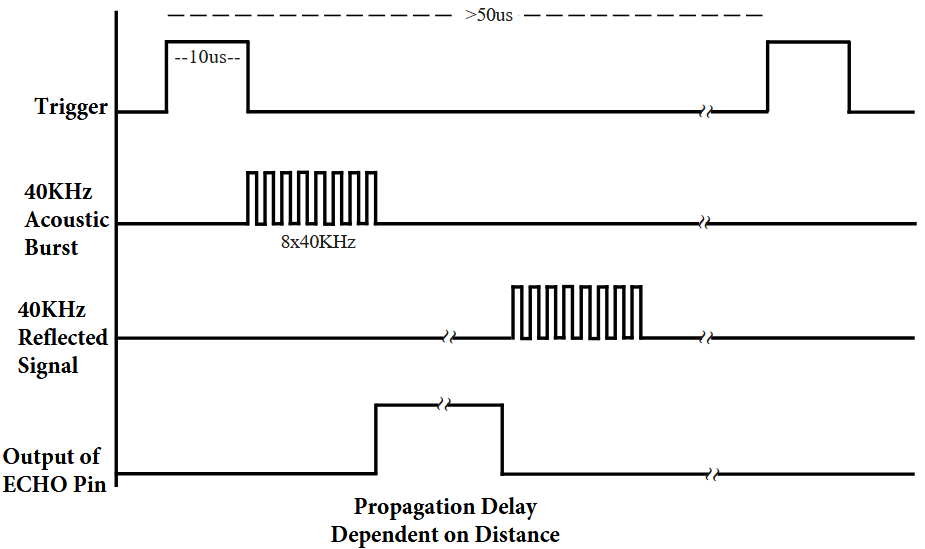
\includegraphics[width=0.8\linewidth]{obrazky-figures/us.png}
    \caption {Princip fungování senzoru HC-SR04, dostupné z: \cite{ultras}}
    \label{ultra_s}
\end{figure}

\section{Motory}
Motory hrají v problematice balancujících robotů zásadní roli -- aplikují kroutící moment, kterým udržují robota ve stabilizované poloze. Je potřeba zvolit správnou variantu, která nabízí dostatečnou sílu a zároveň efektivitu. Aby mohl robot provádět přesné manévry, jako třeba rotace o určitý úhel, musí motor nabízet možnost sledovat, o kolik se jeho osa otočila. V této podkapitole probereme možné varianty motorů, jejich výhody a nevýhody pro tento konkrétní projekt.

Správný výběr kol je neméně důležitý. Aby se robot dokázal zdvihnout ze stabilní polohy, musí kola nabízet vysokou přilnavost. Se zmenšujícím se poloměrem kola klesá kroutící moment, který je potřebný k balancování. Větší poloměr kol zase nabízí lepší průchodnost překážkami. Dostatečný poloměr kola je zásadní, pokud má mít robot schopnost zdvihu ze stabilní polohy -- vnější okraj kol musí ve stabilní poloze přesahovat boční konstrukci rámu a být kontaktním bodem se zemí, viz obrázek \ref{wheel_size}.

\begin{figure}[H]
    \centering
    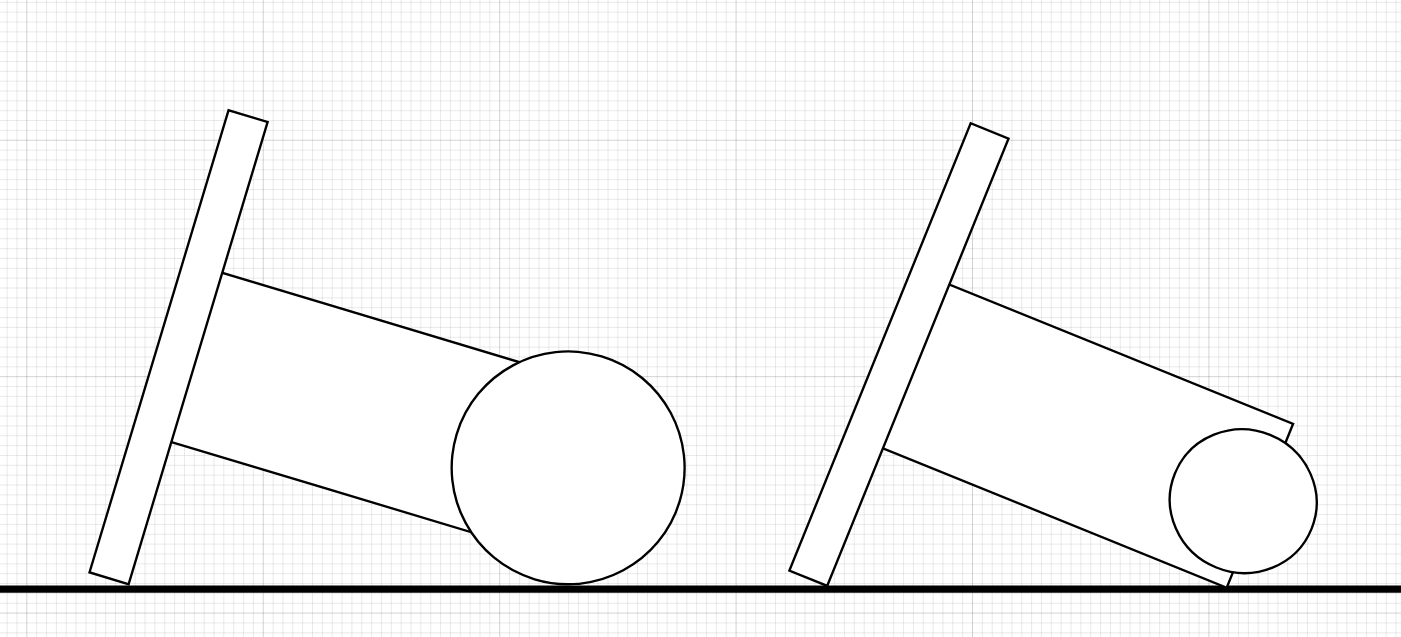
\includegraphics[width=1\linewidth]{obrazky-figures/wheel_size.png}
    \caption {Vlevo je robot s dostatečně velkým kolem schopný zdvihu ze stabilní polohy. Robot vpravo takového manévru kvůli malému poloměru kola schopen není. }
    \label{wheel_size}
\end{figure}

\subsection*{Zvolená varianta}
Jako pohon robota byl zvolen 12V kartáčový stejnosměrný motor. Hlavním důvodem byla zkušenost s motorem v jiném projektu -- motor byl tím pádem k dispozici. Při napětí 12V nabízí až 143 otáček za minutu a dokáže vyvinout kroutící moment 0.55~Nm. Motor je vybaven enkodérem pracujícím na principu Hallova jevu. V dokumentaci výrobce je uvedena přesnost enkodéru jako 663 PPR (pulzy za rotaci), ale vlastním měřením byla tato přesnost určena jako 734 PPR. Maximální proud odebíraný motorem je 3.6~A.

K motoru byla vybrána gumová kola s poloměrem 68 mm a šířkou 24 mm. Díky dostatečné šířce a přilnavému povrchu kola neprokluzují a dokážou efektivně přenést sílu na zem.

K motorům byly také zakoupeny adaptéry na enkodér, díky kterým lze enkodér snadno připojit k Raspberry. Adaptér má zabudovaný pull--up rezistor, který napomáhá k čistému výstupnímu signálu.

Motory jsou na schématu zapojení znázorněny pod písmenem~D a adaptér pod písmenem~E \ref{schema}.

\begin{figure}[H]
  \centering
  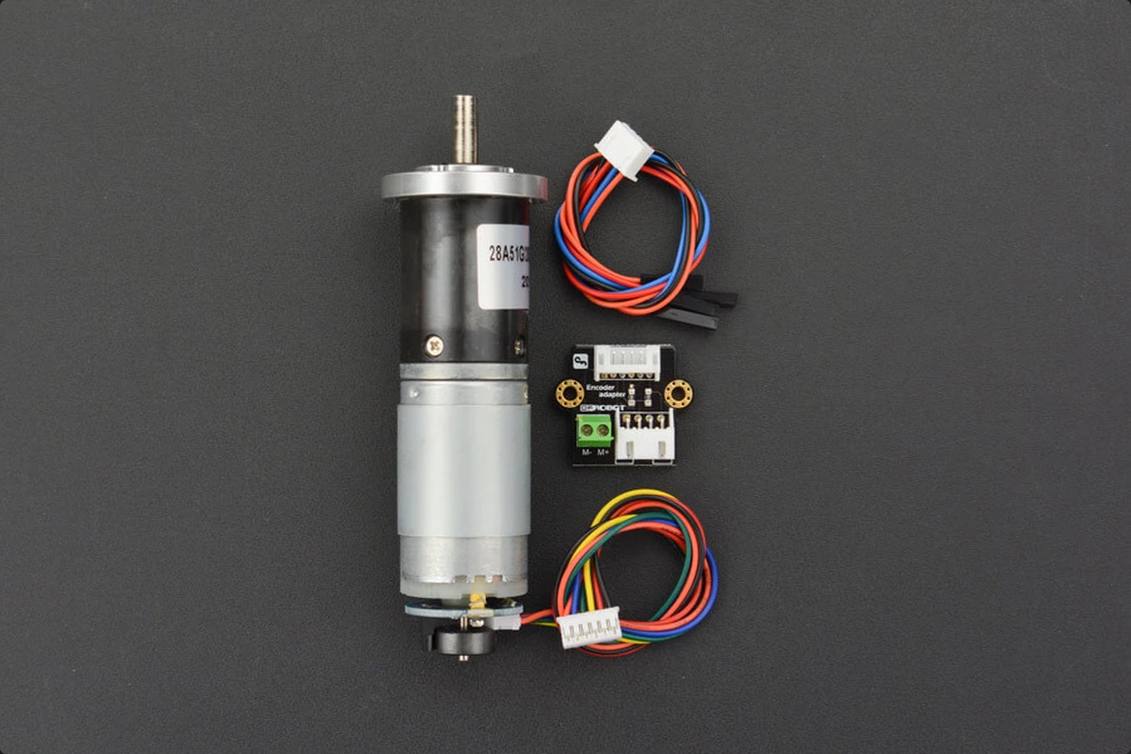
\includegraphics[width=0.5\linewidth]{obrazky-figures/motor.png}\hfill
  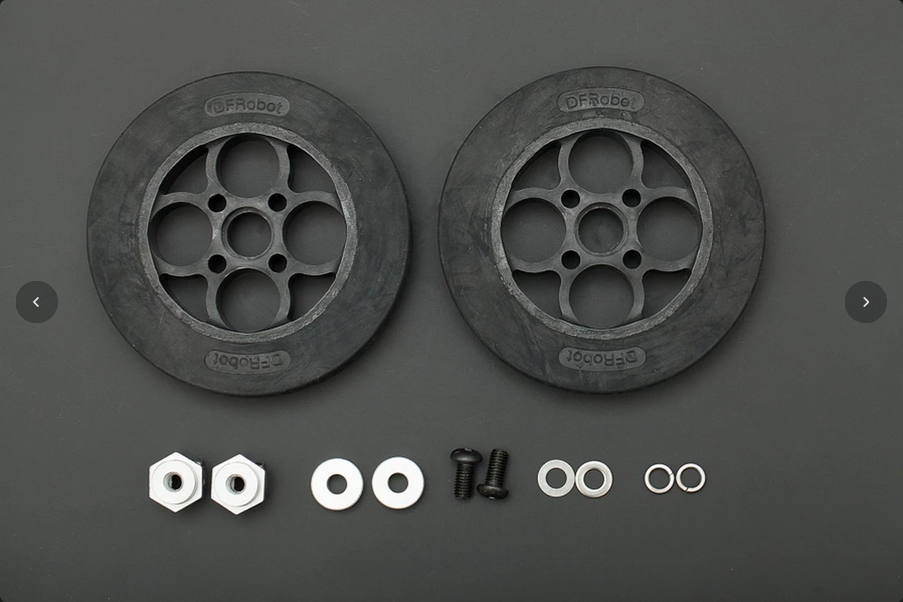
\includegraphics[width=0.5\linewidth]{obrazky-figures/wheel.png}
  \caption{Zvolená varianta motoru a kola, dostupné z \cite{motor_kolo}}
  \label{motor_kolo}
\end{figure}


\subsection*{Řadič motoru}
\label{driver_sec}
Řadič motoru ovládá jakým směrem a s jakou silou se motory otáčí. Z tohoto důvodu bylo nutné vybrat takový řadič, který dokáže zvládnout proud alespoň 3.6~A na jeden kanál.

Zvolen byl model 7A/160W Dual H-Bridge Motor Controller od firmy Handson Technology, který má podle specifikace výrobce zvládnout proud až 7A na kanál a doručit napětí až 24~V. Každý kanál má 3 ovládací vstupy: PWM, IN1 a IN2. Vstup PWM (Pulse-width modulation, česky Pulzně šířková modulace) určuje sílu otáčení motoru pomocí nastavování střídy signálu. Kombinací vstupů IN1 a IN2 lze měnit směr otáčení a používat režimy brždění a volného otáčení. \cite{driver1}

Řadič se bohužel ukázal jako nekvalitní, kdy u prvního kusu po krátkém čase přestal fungovat kanál číslo 2. U druhého kusu se zase projevila vada s nerovnoměrným výstupem z kanálů 1 a 2 při stejné vstupní PWM hodnotě -- na výstupu kanálu 1 bylo pomocí multimetru naměřeno vyšší napětí než na výstupu kanálu 2, což vedlo k rozdílné síle motorů.

Vadný model byl nahrazen byl nahrazen jiným řadičem -- kvůli nedostupnosti vhodných alternativ značně předimenzovaným MDD20A od výrobce CYTRON. Ten dokáže na jeden kanál vysílat nepřetržitě 20~A napětí (ve špičce až 60~A) a dokáže doručit napětí až 30V. Na rozdíl od předchozího řadiče nabízí MDD20A nadproudovou a teplotní ochranu. Je také vybaven čtyřmi testovacími tlačítky (dvě na kanál), pomocí kterých lze ovládat motory i bez PWM signálu z řídící desky. \cite{driver2} Nevýhodou řadiče oproti předchozímu je mnohonásobně vyšší cena, absence režimu volného otáčení a také větší rozměry. Ukázka zapojení a ovládací tabulky je na obrázku \ref{driver}.

Řadič motoru je na schématu zapojení znázorněn pod písmenem~G \ref{schema}.

\begin{figure}[H]
    \centering
    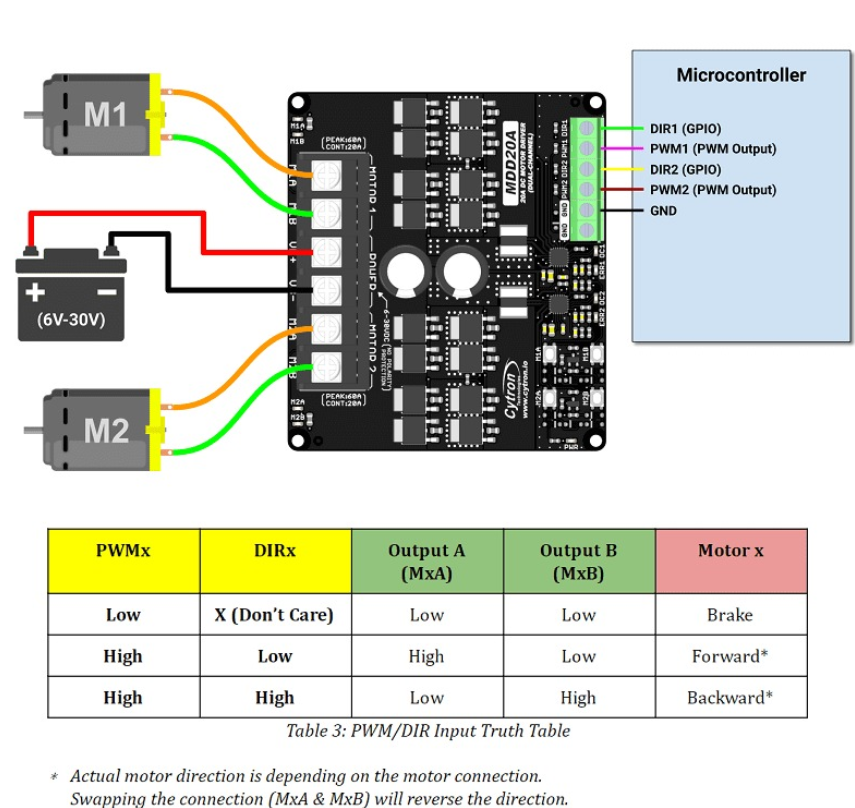
\includegraphics[width=0.9\linewidth]{obrazky-figures/driver.png}
    \caption {Řadič motorů MDD20A s ukázkou zapojení motorů a mikrokontroléru. Ve spodní části obrázku je pravdivostní tabulka s možnými kombinacemi vstupní logiky. Obrázek je převzat z \cite{driver2} }
    \label{driver}
\end{figure}


\section{Napájení}
Baterie zajišťuje mobilitu robota. Je nutné, aby dokázala dodávat napětí okolo 12V, měla vybíjecí proud alespoň 10.2~A (každý motor 3.6~A, Raspberry Pi 3~A) a zároveň dostatečnou kapacitu. Baterii je potřeba nabíjet bez nutnosti vyjmutí z robota.

\subsection*{Zdroj a balancér}
Zdroj se skládá ze šesti Li-Ion 18650 baterií výrobce MOTOMA.  Konstantní napětí baterie je 4.2~V, kapacita 2500~mAh. Baterie má velmi vysoký nepřetržitý vybíjecí proud 5C, což znamená, že za hodinu dokáže bezpečně vybít pětinásobek své kapacity.

Baterie jsou zapojeny v konfiguraci 3S2P -- dvě baterie paralelně třikrát v sérii. Díky tomu zdroj dosahuje maximálního napětí 12.6~V a vybíjecího proudu až 25~A. Kapacita zdroje je 5000~mAh.

Zdroj má zabudovaný balancér, který zajišťuje rovnoměrné nabíjení mezi jednotlivými články. Obsahuje ochranu proti zkratu, přetížení a vybití pod únosnou mez. Balancér byl vybrán, protože má dostatečně vysoký vybíjecí proud (40~A -- vyšší než vybíjecí proud zdroje) a kvůli podpoře zapojení 3S2P.

Zdroj a balancér je na schématu zapojení znázorněn pod písmenem~A \ref{schema}.

\begin{figure}[H]
    \centering
    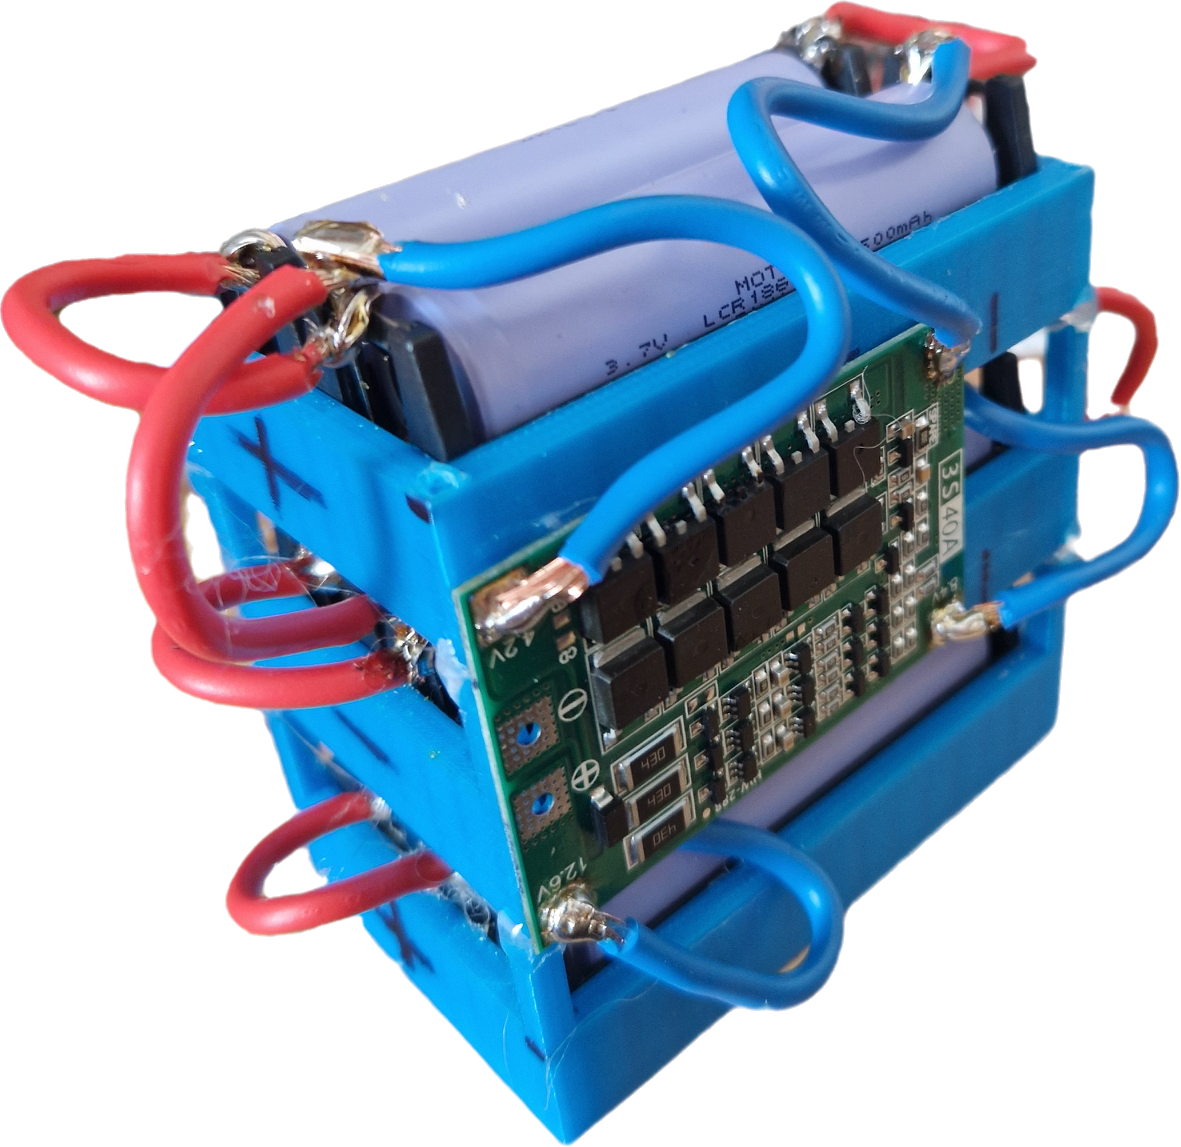
\includegraphics[width=0.6\linewidth]{obrazky-figures/battery.png}
    \caption {Baterie a balancér}
    \label{baterie}
\end{figure}

\subsection*{USB-C modul}
Jako nabíjecí konektor byl zvolen ZY12PDN USB-C modul. Podporuje standarty Power Delivery 2.0 a 3.0, díky kterým dokáže s vhodnou nabíječkou dodávat napětí až 20~V. V projektu se používá ve 12V režimu. Modul má zabudovanou LED diodu, která signalizuje, v jakém režimu modul pracuje.

Modul měl zpočátku problém dodávat jiné napětí, než výchozích 5V i přesto, že byla zvolená kompatibilní nabíječka. Modul je totiž připojen na step-up měnič (viz schéma), který však propouštěl velmi nízké napětí (okolo 0.15~V) směrem od baterie k USB-C. To znemožnilo USB modulu dojednat přes Power Delivery protokol vyšší napětí. Problém byl vyřešen připájením rezistoru s vysokým odporem (10~k$\Omega$) přes póly USB modulu.

USB-C modul je na schématu zapojení znázorněn pod písmenem~C \ref{schema}.

\subsection*{Konvertory napětí}
Robot používá dva konvertory napětí. Jeden slouží ke zvýšení napětí z 12~V na 12.6~V (Step--up měnič) a druhý snižuje napětí z 12.6~V na 5~V (Step--down měnič).

Step-up měnič se používá pouze při nabíjení. Konkrétní zvolený modul je schopen regulovat vstupní napětí 8.5-48~V na výstupní napětí 12--50~V. Výstupní napětí musí být vždy vyšší než vstupní -- jinak hrozí poškození desky. Z tohoto důvodu nelze nabíjet robota za provozu. Na straně zdroje totiž může být napětí nižší, něž na straně USB-C modulu. V tomto projektu má na vstupu napětí 12~V, které jde z USB-C. Měnič napětí zvýší na 12.6~V, což je maximální kapacita zdroje. Zároveň také omezuje maximální nabíjecí proud na přibližně 2~A, což zamezuje přehřívání součástek a výrazně prodlužuje životnost baterií. \cite{bat_life} Cenou za nižší proud je delší doba nabíjení. Step--up měnič je na schématu zapojení znázorněn pod písmenem~B \ref{schema}.



Step--down měnič slouží ke snížení vysokého napětí ze zdroje na konstatní napětí 5~V, kterým se napájí deska Raspberry Pi. Měnič má vstupní napětí 9--35~V, výstupní je vždy 5~V. Výstupní proud je až 5~A, což pro napájení Raspberry Pi stačí. Step--down měnič je na schématu zapojení znázorněn pod písmenem~F \ref{schema}.

\begin{figure}[H]
    \centering
    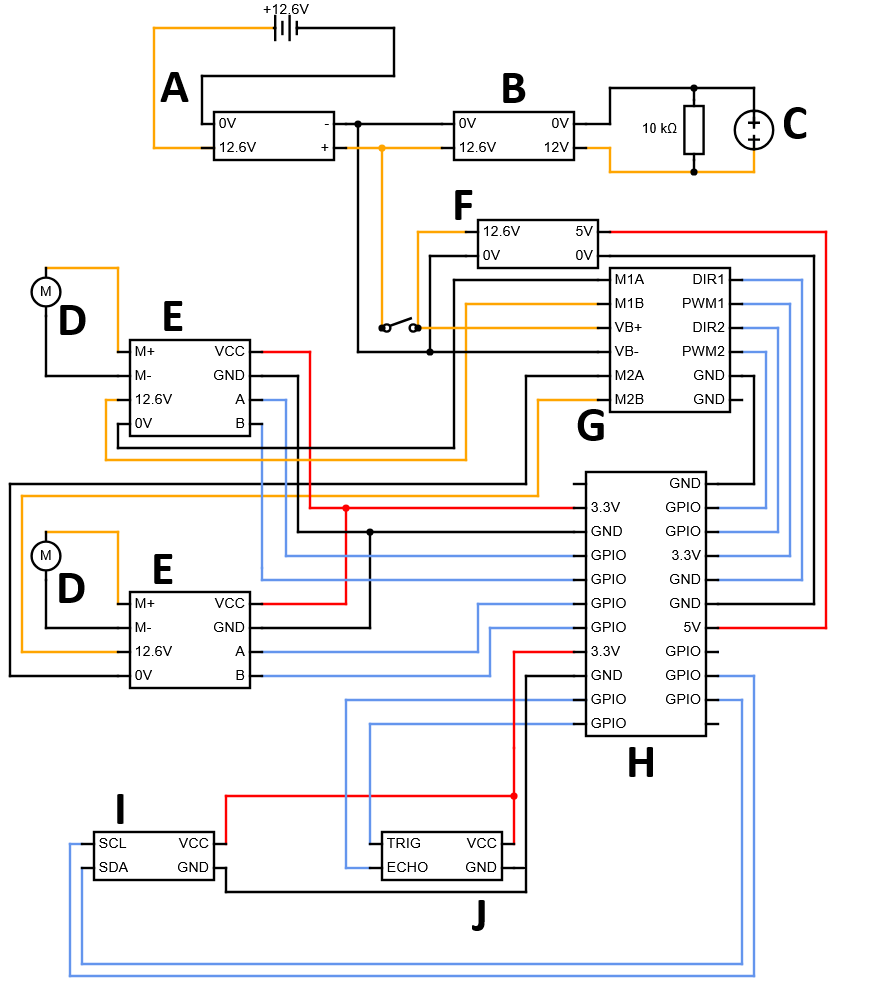
\includegraphics[width=1\linewidth]{obrazky-figures/circ.png}
    \caption {Schéma zapojení robota. \textbf{Legenda}: černý vodič 0~V, oranžový vodič 12~V, červený vodič 3--5~V, modrý vodič data. \textbf{A}: zdroj, \textbf{B}: step-up měnič, \textbf{C}: USB-C modul, \textbf{D}: motory, \textbf{E}: adaptér na motor a enkodér, \textbf{F}: step-down měnič, \textbf{G}: motorový řadič, \textbf{H}: Raspberry Pi 4, \textbf{I}: gyroskop a akcelerometr, \textbf{J}: ultrazvukový snímač. Schéma bylo vytvořeno ve webové aplikaci https://app.smartdraw.com/}
    \label{schema}
\end{figure}


\section{Konstrukce rámu}
Co se výroby rámu robota týká, padla volba na 3D tisk. Díky tomu bylo možné navrhnout konstrukci přesně na míru zvoleným elektronickým součástkám. Konstrukce z materiálu PLA je velmi lehká a zároveň pevná. Jednotlivé díly jsou k sobě připevněny pomocí tavného lepidla.

Návrh jednotlivých dílů probíhal ve webové aplikaci Tinkercad (https://www.tinkercad.com/). Ta nabízí intuitivní rozhraní a snadný návrh designů. Tisk samotný probíhal na tiskárně i3 MK3S od firmy Prusa.

Kvůli ochraně elektroniky proti nárazům má robot ve vrchní části dva nárazníky. Můžeme je vidět na obrázku \ref{robot-side} (šedá ramena v pravé části obrázku). Každý z nich se skládá ze dvou ramen spojených pružinou, která zajistí ztlumení nárazu při pádu. Nárazníky jsou z důvodu lepší přenosnosti robota snadno odnímatelné. 

\begin{figure}[H]
    \centering
    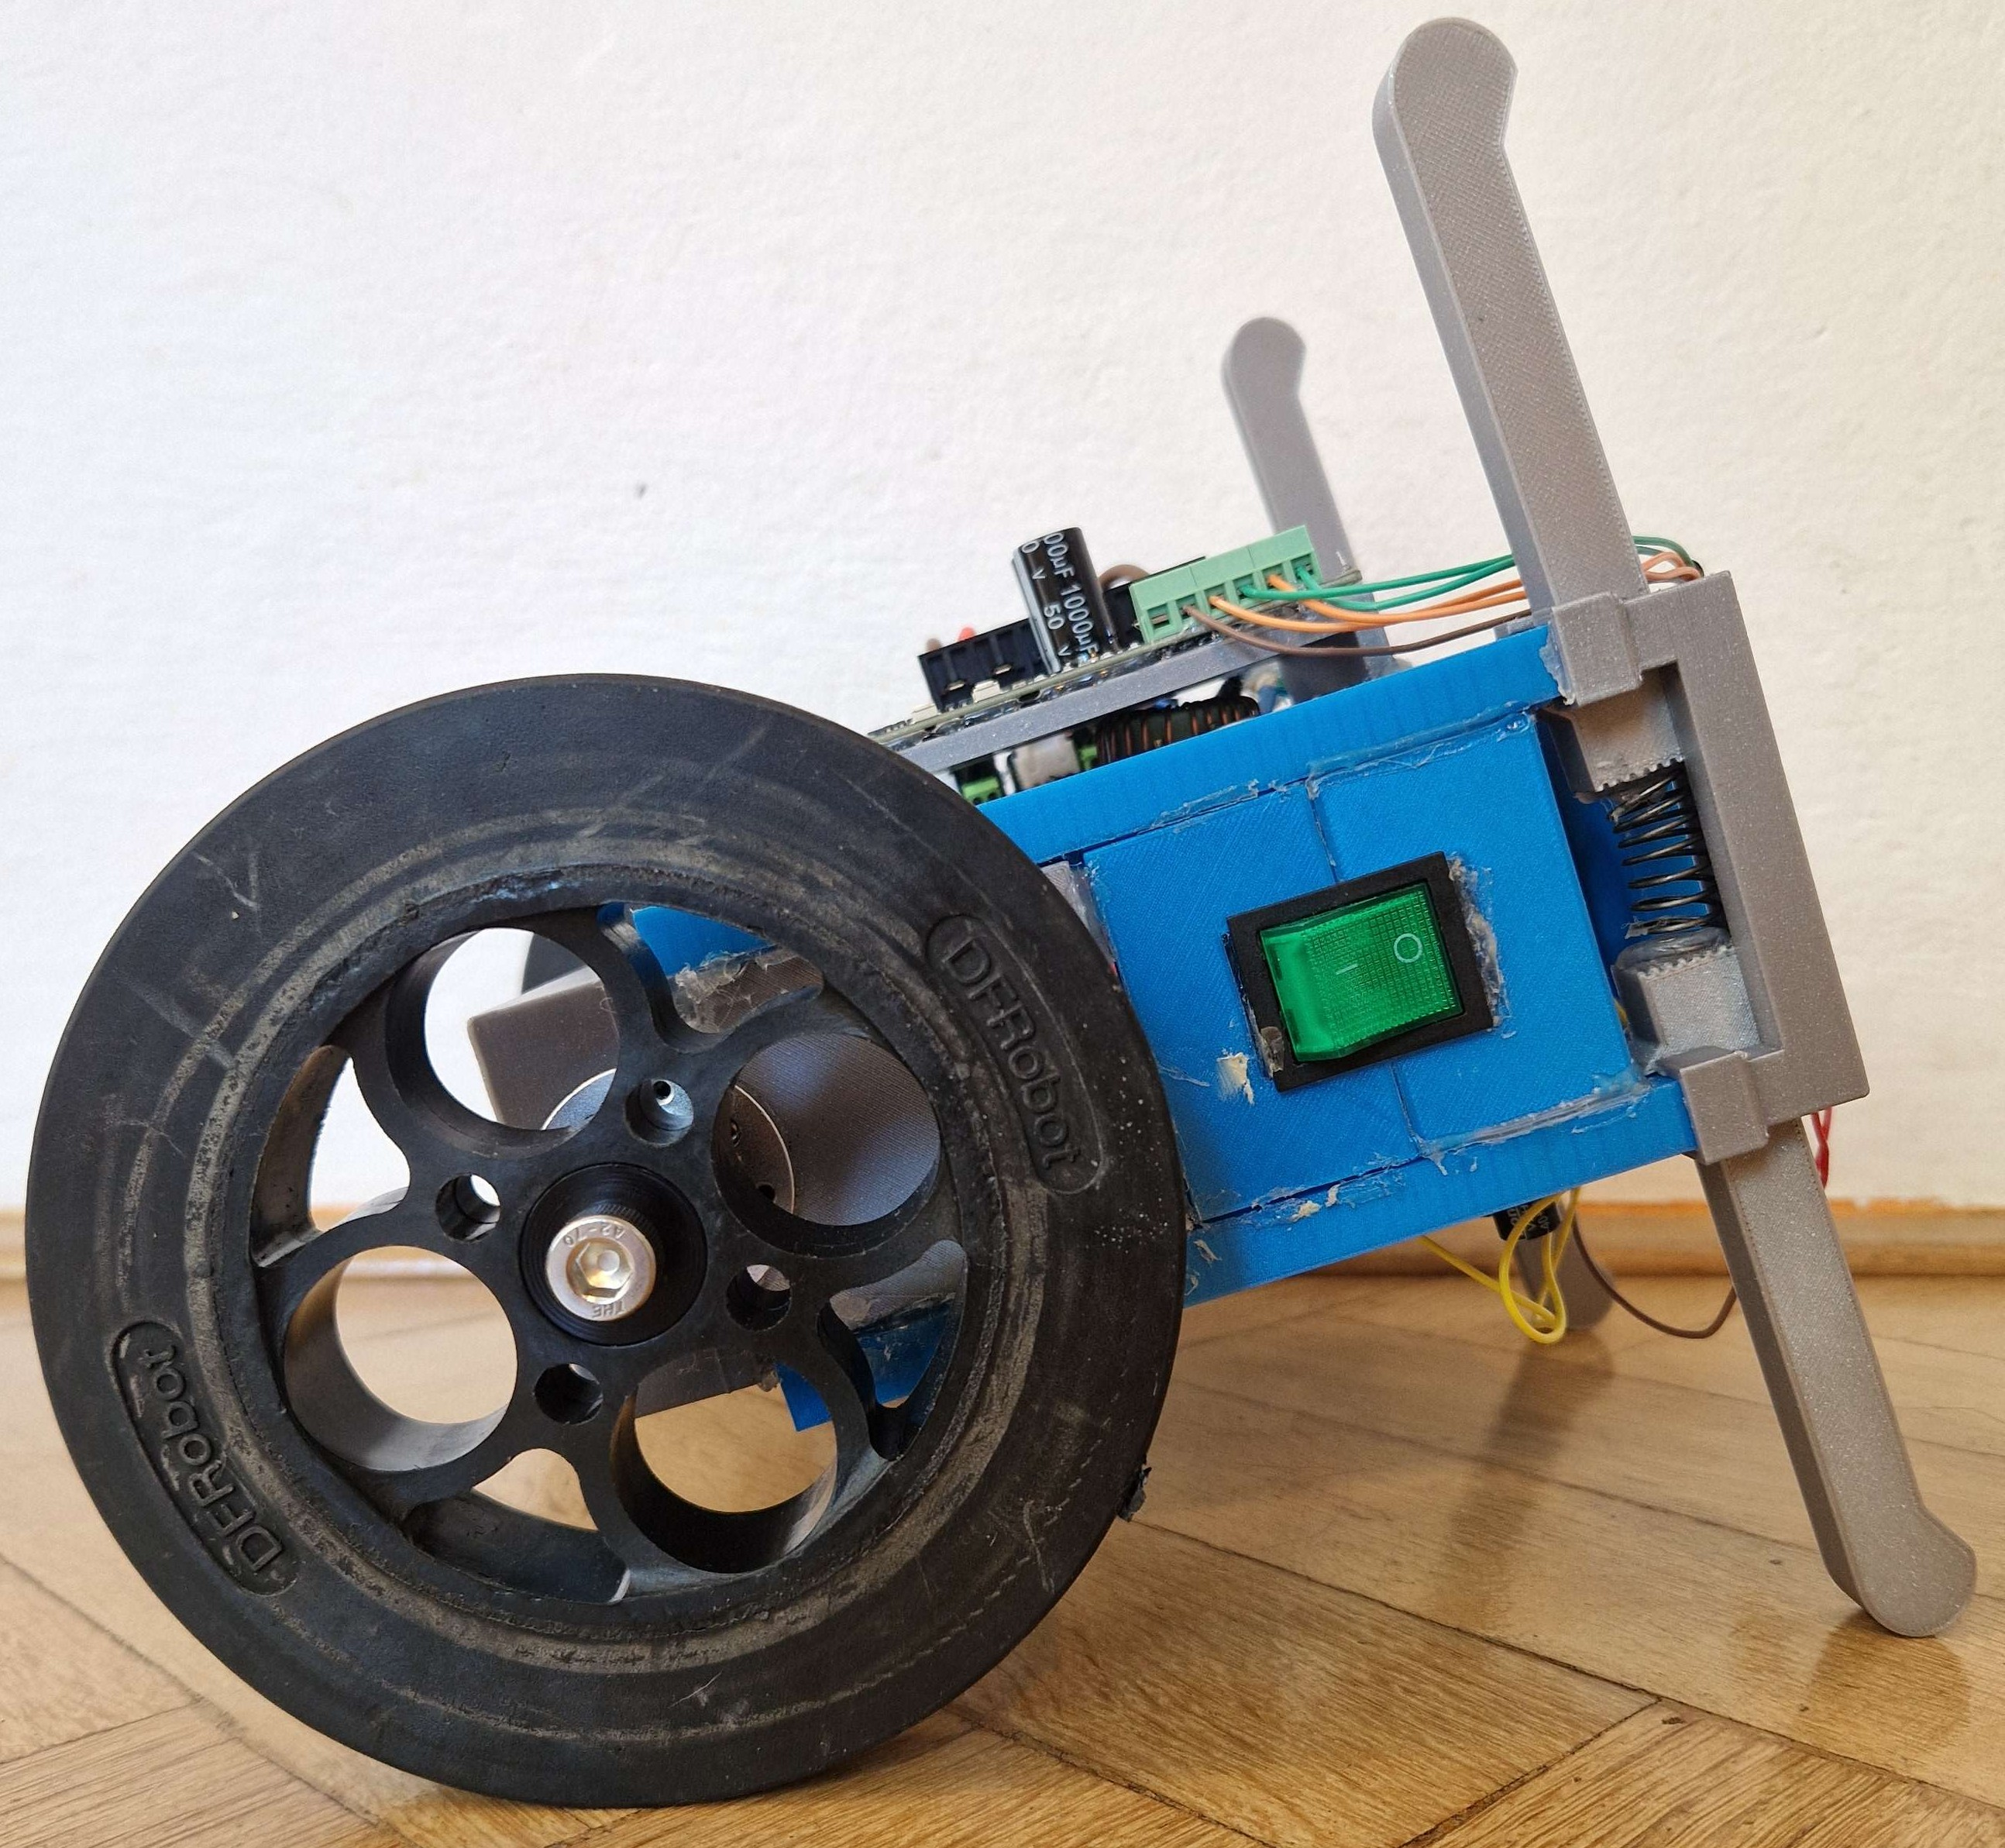
\includegraphics[width=0.9\linewidth]{obrazky-figures/side.jpg}
    \caption {Robot -- pohled z boku}
    \label{robot-side}
\end{figure}

\section{Finální podoba}
Robot i s koly váží 2410~g a měří 27~cm. Motory jsou uloženy v základně, 2~cm nad nimi je připevněný gyroskop/akcelerometr. Nad ním je zdroj, který má z jedné strany připevněný balancér baterie a z druhé strany step--up měnič.

Kvůli neplánované změně řadiče (viz \ref{driver_sec}) muselo dojít ke změně konstrukce -- nový řadič je výrazně větší než starý. Místo původního umístění uvnitř konstrukce je nový řadič umístěn nad step--up měničem, protože by se dovnitř bez zásadní změny konstrukce nevešel. To způsobuje nevyváženost v konstrukci, kdy je těžiště robota vychýleno na stranu, kde se nachází tento řadič. To se při balancování musí následně kompenzovat vychýlením cílového úhlu na opačnou stranu. Aby se zabránilo škodě při případném nárazu, je platforma pro řadič připevněna k robotovi pouze na horní straně a je tím pádem pružná.

Raspberry Pi je z důvodu snadnější manipulace s rozhraním GPIO umístěno na vrchní straně robota.

Tavné lepidlo se později ukázalo jako špatná volba -- obtížně se odstraňuje, když je potřeba přístupu k vnitřním komponentám. Musí se nahřát, což ale poškozuje plastovou konstrukci, která se deformuje. Vhodnější variantou by byla šroubovaná 3D vytisknutá konstrukce.

\begin{figure}[H]
    \centering
    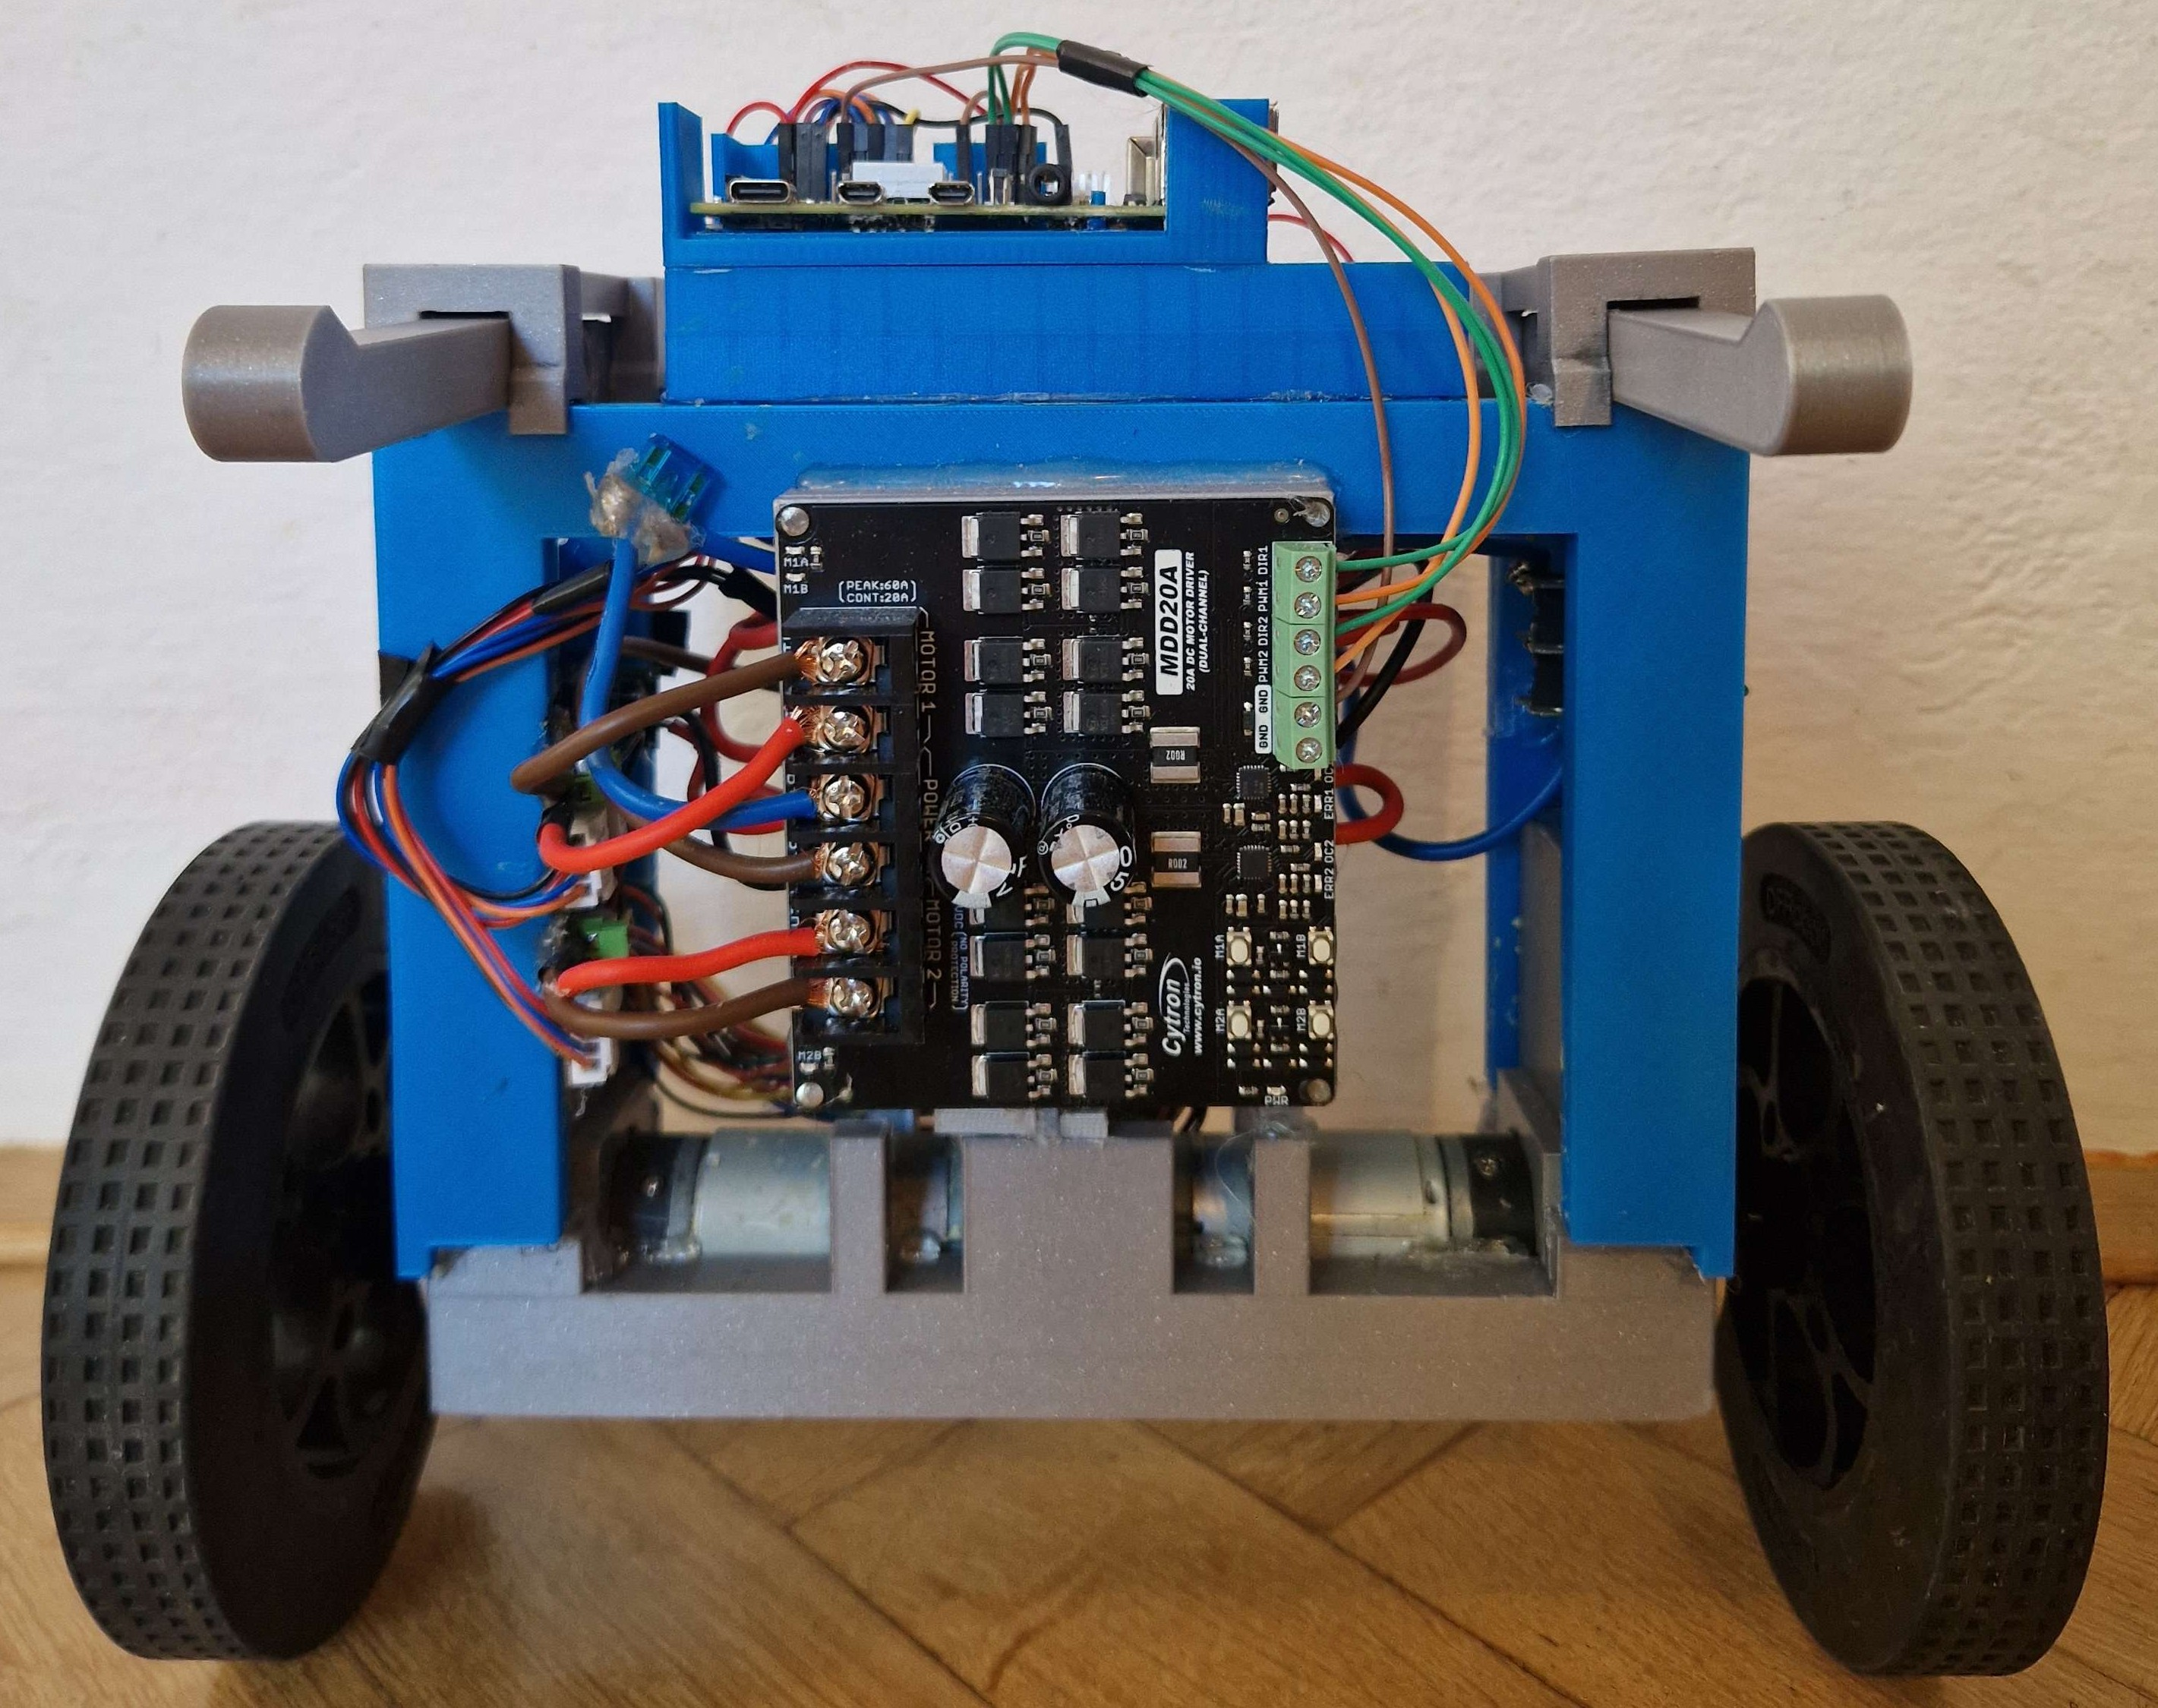
\includegraphics[width=0.9\linewidth]{obrazky-figures/front.jpg}
    \caption {Robot -- pohled zpředu. V základně robota vidíme uložení dvou DC motorů, které zabírají celou šířku základny. Nad nimi je jejich řadič. Na vrchní straně robota je řídící jednotka Raspberry Pi4B.}
    \label{robot-front}
\end{figure}

\begin{table}[H]
	\vskip6pt
	\caption{Cena komponent (uvedeno bez dopravy a dodatečného cla za produkty zakoupené mimo EU} 
    \vskip6pt
	\centering
	\begin{tabular}{lrrr}
		\toprule
		Komponenta & Množství & Cena za kus (Kč) & Cena celkem (Kč) \\
		\midrule
        Řídící jednotka & $1$ & $1164$ & $1164$ \\
		Motor & $2$ & $857$ & $1714$ \\
        Kolo (set) & $1$ & $659$ & $659$ \\
        Adaptér na enkodér & $2$ & $77$ & $154$ \\
        Řadič motorů & $1$ & $825$ & $825$ \\
        MPU & $1$ & $68$ & $68$  \\
        USB-C modul & $1$ & $168$ & $168$ \\
        Baterie & $6$ & $129$ & $774$ \\
        Bateriové pouzdro & $6$ & $25$ & $150$ \\
        Ochrana a balancér baterie & $1$ & $48$ & $48$ \\
        Step-up měnič & $1$ & $138$ & $138$ \\
        Step-down měnič & $1$ & $89$ & $89$ \\
        Přepínač kolébkový & $1$ & $28$ & $25$ \\
        Ultrazvukový měřič vzdálenosti & $1$ & $38$ & $38$ \\
        Přepínač kolébkový & $1$ & $28$ & $28$ \\
        Filament PRUSA PLA 1kg & $1$ & $699$ & $699$ \\
        \midrule
        \textbf{Celkem} & & & \textbf{6741} \\
		\bottomrule
	\end{tabular}
	\label{tab:ExampleTable}
\end{table}


\chapter{Software a implementační detaily}
\label{chap5}
V této kapitole je popsán postup, jakým se čtou a zpracovávají data ze senzorů a jaké je nastavení operačního systému. Dále je zde popis užití systému ROS2, implementace balančního mechanismu a ovládání robota.

\section{Ubuntu, RT KERNEL}
\label{system}
Jako operační systém pro Raspberry bylo zvoleno Ubuntu 22.04 LTS, protože podporuje zvolenou distribuci ROS2 Humble. Projevil se ovšem problém velmi pomalého startu (obvykle přes minutu), což pro robotickou platformu není ideální. Systém navíc neměl jádro běžící v reálném čase, stávalo se tedy, že proces operačního systému (nesouvisející s programem robota) měl vysokou prioritu a na krátký moment zpomalil, nebo úplně zastavil průběh balancování. To obvykle vedlo k pádu robota.

Řešení tohoto problému bylo nainstalovat verzi Linuxu se sadou úprav jádra \textbf{PREEMPT\_RT}. Ze zdroje \cite{RT_source} byla stažena verze operačního systému Ubuntu Server 22.04.5, která obsahuje právě jádro s úpravou \textbf{PREEMPT\_RT} určenou přímo pro Raspberry Pi4. Navíc má systém už předinstalovaný ROS2 Humble. Takto modifikovaný systém sice stále nemá přesně deterministické chování, jako například platforma Arduino, ale jde o výrazně zlepšení proti Ubuntu se standardním jádrem. \cite{RT}

Operační systém Ubuntu ve verzi \textbf{Server} nemá grafické rozhraní a oproti verzi \textbf{Desktop} nemá v základu nainstalované téměř žádné aplikace. To výrazně přispělo k rychlejšímu startu systému -- podle vlastního měření šlo o přibližně 70 sekund ve verzi Desktop a přibližně 30 sekund ve verzi Server. \cite{server}

\section{Robot operating system 2}
ROS2 (Robot Operating System 2) je open-source framework pro tvorbu robotických aplikací. Pro projekty nabízí vysokou modularitu a škálovatelnost. Jde o vývoj systému ROS1, oproti kterému novější verze přináší například podporu programů, které běží v reálném čase, nebo nastavení QoS (Quality of service -- kvalita služeb), díky kterému si lze pro přenos dat v projektu zvolit mezi garancí dodání dat a nízkou latencí.

Projekt v ROS2 je rozdělen do \textbf{balíčků} (package), což jsou adresáře obsahující všechny potřebné soubory (zdrojový kód, konfigurační soubory, metadata) pro jednu oblast zaměření projektu. Jeden balíček může obsahovat několik \textbf{uzlů} (node) s podobným zaměřením. Uzel obvykle zajišťuje jednu specifickou funkcionalitu projektu. ROS2 poskytuje standardizovaný způsob komunikace mezi uzly, pomocí takzvaných \textbf{témat} (topic). Uzel může tato témata \textbf{odebírat} (subscriber) a \textbf{zveřejňovat} (publisher).

\subsection*{Použití ROS2 v projektu}
Projekt balancujícího robota je v ROS2 rozdělen do čtyř balíčků. Každý z nich obsluhuje jednu oblast. 

\begin{enumerate}
  \item{\textbf{Sensors\_pkg} obsahuje uzly, které se starají o čtení a zpracování dat ze senzorů -- \it encoder\_node \rm čte data z enkodŕů motorů, \it imu\_node \rm čte a zpracovává data z akcelerometru a gyroskopu a \it ultra\_s\_node \rm čte data z ultrazvukového senzoru a určuje vzdálenost překážek. Uzly z tohoto balíčku zveřejňují data, která následně odebírá uzel \it motor\_controller\_node \rm. }
  \item{\textbf{Bluetooth\_pkg} obsahuje uzel \it bluetooth\_node \rm, který obsluhuje komunikaci s mobilním telefonem. Pomocí balíčku BlueDot zajišťuje dálkové ovládání a komunikaci s aplikací na telefonu.}
  \item{\textbf{Control\_pkg} obsahuje uzel \it motor\_controller\_node \rm, interpretující data ze senzorů a vypočítávající potřebnou reakci motorů.}
  \item{\textbf{Robot\_bringup} obsahuje uzel \it robot\_bringup \rm, který se stará o korektní spuštění celého projektu.}
\end{enumerate}

\begin{figure}[H]
    \centering
    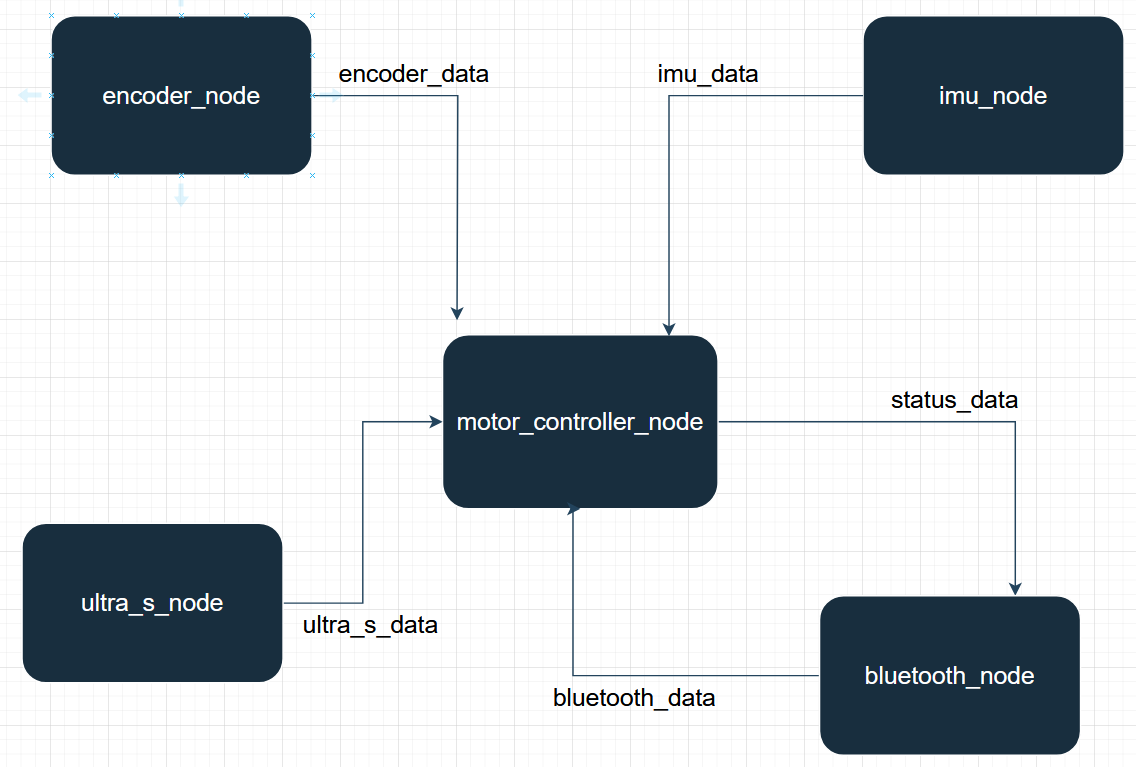
\includegraphics[width=1\linewidth]{obrazky-figures/ros_graph.png}
    \caption {Graf projektu v ROS2, vytvořeno nástrojem https://app.diagrams.net}
    \label{motor}
\end{figure}

\section{Data ze senzorů}

\subsection*{Čtení a zpracování dat enkodérů}
Motory jsou vybaveny enkodéry, které pracují na principu Hallova efektu. Každý z nich má dva datové výstupy -- \textbf{A} a  \textbf{B}. Výstup A obstarává přerušení (interrupt). V programu je nutné nastavit, jaký druh přerušení budeme detekovat -- rostoucí hrana (rising edge), klesající (hrana) nebo obě. Sledování obou hran nabízí vyšší přesnost, ale má vysoké nároky na schopnost systému zpracovávat přerušení v reálném čase. 

Enkodéry mají výrobcem definovanou přesnost. V případě modelu použitém v robotovi je to 734 PPR (pulzy za otočku) -- to znamená, že za jednu kompletní rotaci motoru by měl enkodér vyslat přesně tolik přerušení (dvakrát víc, pokud používáme detekci obou hran). Ve chvíli, kdy systém obdrží přerušení, musí přečíst stav výstupu \textbf{B}. Ten obsahuje informaci, jakým směrem se motor točí. 

Čtení enkodérů je v robotovi realizováno pomocí knihovny \textbf{libgpiod}. Na rozdíl od knihovny \textbf{pigpio} (kterou používají pro čtení vstupu a vytváření výstupu ostatní uzly) je tato lépe uzpůsobena pro  použití v systému s plánováním v reálném čase. Při prodlevě čtení může dojít k situaci, kdy přijmeme přerušení v signálu \textbf{A}, ale než program stihne přečíst stav signálu \textbf{B}, hrana může být už v jiné poloze -- viz obrázek \ref{enc}.

Aby se toto zpoždění minimalizovalo, je potřeba uzlu nastavit vysokou prioritu v systémovém plánovači. To zajišťuje funkce \textbf{set\_realtime\_priority} (viz níže \ref{prio}). Priorita se nastaví na hodnotu 81 (z rozsahu 0--99, kde 0 je nejnižší priorita), což je nejvíce ze všech běžících uzlů projektu.

\begin{verbatim}
void set_realtime_priority() {
    struct sched_param sched;
    sched.sched_priority = 81;
    if (pthread_setschedparam(pthread_self(), SCHED_FIFO, &sched)) {
        perror("Failed to set real-time priority");
    }
}
\end{verbatim}
\label{prio}

\begin{figure}[H]
    \centering
    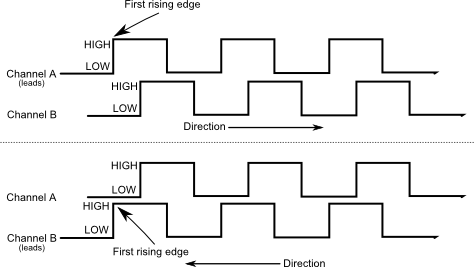
\includegraphics[width=0.7\linewidth]{obrazky-figures/edges.png}
    \caption {Výstup enkodéru, převzato z \cite{encoder}}
    \label{enc}
\end{figure}

I po nastavení vysoké priority měl program problém číst výstup z enkodéru, pokud měl motor vysoké otáčky. Program sice korektně přečetl přerušení, ale čtení směru bylo velmi chaotické. To vedlo k chybnému určení vzdálenosti, o kterou se kolo otočilo. Aby čtení enkodéru získalo ještě vyšší prioritu, bylo mu nakonec přiděleno celé jádro procesoru. Úpravou konfiguračního souboru \it /boot/cmdline.txt \rm bylo nastaveno, aby plánovač operačního systému nepoužíval jádro číslo 3. Samotný ROS2 uzel obstarávající čtení enkodérů je spuštěn s příkazem \it taskset -c 3 \rm, který uzel spustí na exkluzivně přiděleném jádru 3.

Výsledek úpravy je vidět na obrázku \ref{enc_bad}, kde je zaznamenán relativní rozdíl mezi enkodéry v průběhu času. Experiment neukáže přesnou chybu enkodéru (rozdíl může být způsobený zpomaleným čtením jednoho či zrychleným čtením druhého enkodéru), ale nastíní, jak špatné nastavení priority u citlivých procesů ovlivní čtení dat. Nahoře vidíme vznikající rozdíl mezi enkodéry 1 a 2 ve chvíli, kdy se obě kola točí konstantní rychlostí 100 otáček za minutu. Rychlé skoky jsou místa, kdy bylo čtení přerušení zpomaleno jiným procesem. Vidíme, že v průběhu jedné minuty se rozdíl mezi enkodéry 1 a 2 přiblížil k hodnotě 3000, což je při přesnosti 734 pulzů za otáčku rozdíl asi čtyř celých rotací motoru. 

Na druhém obrázku \ref{enc_good} je stejné měření, pouze v tomto případě běží ROS2 uzel na exkluzivním jádru procesoru a tím pádem ho neovlivňuje běh systému. V průběhu minutového měření chyba dosáhla hodnoty nejvýše 60 pulzů, což mohlo být způsobeno přímo motorem (například krátký pokles napětí v jednom motoru).

\begin{figure}[H]
    \centering
    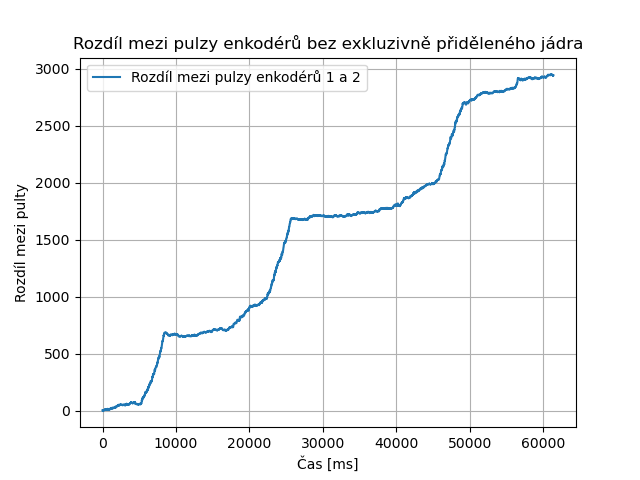
\includegraphics[width=0.8\linewidth]{obrazky-figures/bad.png}
    \caption {Měření bez exkluzivního jádra}
    \label{enc_bad}
\end{figure}

\begin{figure}[H]
    \centering
    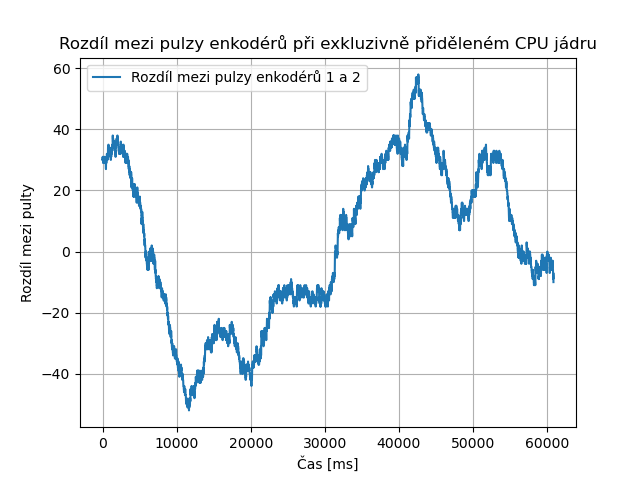
\includegraphics[width=0.8\linewidth]{obrazky-figures/good.png}
    \caption {Měření s exkluzivním jádrem}
    \label{enc_good}
\end{figure}

Výstupem uzlu \textbf{encoder\_node}, který zajišťuje zpracování dat z enkodérů, jsou hodnoty \it rpm1 \rm a \it rpm2 \rm. Každá z nich obsahuje počet pulzů motoru, ke kterému daný enkodér patří.

\subsection*{Čtení a zpracování dat z gyroskopu a akcelerometru}
Příjem dat z gyroskopu a akcelerometru (dále IMU) je realizován pomocí sběrnice I²C. Nejdříve bylo měření úhlu náklonu realizováno pomocí knihovny \textbf{wiringPi}. Úhel náklonu byl z dat IMU vypočítán pomocí komplementárního filtru, viz \ref{compl}. Toto řešení nicméně trpí na silný šum ve výsledcích a hlavně na dekalibraci při běhu programu. To ve výsledku znamená, že měření se v průběhu stávalo méně a méně přesné.

\begin{verbatim}
alpha = 0.98
angle = alpha * (angle + gyroRate * delta_time) + (1 - alpha) * accelAngle;
\end{verbatim}
\label{compl}

Řešením problému je knihovna \textbf{RTIMULib.h} \cite{RTIMULib}. Ta sama obstarává čtení dat z IMU a není na to potřeba dalších knihoven (jako wiringPi nebo pigpio). Knihovna používá pokročilé filtry na určování úhlu náklonu -- v případě tohoto projektu se jedná o Kálmánův filtr. Nabízí také možnost kalibrace senzoru před provozem. Při běhu programu se oproti komplementárnímu filtru ztrácí přesnost výrazně pomaleji.

Výstupem uzlu \textbf{IMU\_node}, který zajišťuje zpracování dat z IMU, jsou hodnoty \it tilt \rm a \it velo \rm. Tilt obsahuje současný úhel náklonu robota (ve stupních). Velo obsahuje úhlovou rychlost robota (ve stupních za sekundu).

\subsection*{Čtení a zpracování dat z ultrazvukového snímače}
Ultrazvukový měřič vzdálenosti pracuje v režimu \textbf{1Wire}, což znamená, že nepoužívá ke komunikaci s řídící jednotkou rozhraní I²C či UART, ale pracuje přímo s logickou hodnotou na příslušném GPIO pinu. Čtení a zápis hodnot na GPIO je obstaráno knihovnou \textbf{pigpio}. Vzdálenost od překážky se určuje měřením, za jak dlouho se vrátí vyslaná zvuková vlna. Podrobněji je fungování probráno v kapitole \ref{ultra_s}.

Snímací frekvence je 10 Hz. Pokud výsledek snímání ukazuje výrazný výkyv od posledního výsledku, je označen za falešný a nepoužije se. 5 posledních získaných hodnot se ukládá do pole, ze kterého se následně počítá průměr. Toto filtrování je nutné kvůli nižší spolehlivosti senzoru.

\section{Balancování}
\label{balanc}

Balancování robota zajišťují dva PID regulátory -- \textbf{vnější} a \textbf{vnitřní}. Vnitřní z úhlu náklonu a z úhlové rychlosti vypočítává nutnou reakci motorů, vnější podle dat z enkodérů určuje, vychýlení z výchozí polohy a posílá nutnou korekci do vnitřní smyčky.

Další PID regulátor je \textbf{směrový}. Na vstupu má chybu mezi pulzy z enkodérů jednotlivých motorů a vypočítává nutnou reakci ke srovnání tohoto rozdílu.

Všechny tři regulátory pracují na frekvenci 100 Hz a jsou na sebe přímo navázané. Návaznost je znázorněna na obrázku \ref{PID}. Jednotlivé koeficienty jsou v tabulce \ref{coeffs}.

\begin{table}[H]
	\vskip6pt
	\caption{Koeficienty vnějšího a vnitřního PID regulátoru} 
    \vskip6pt
	\centering
	\begin{tabular}{lrrr}
		\toprule
		Smyčka & Kp & Ki & Kd \\
		\midrule
        Vnější & $0,006$ & $0,008$ & $0,007$ \\
		Vnitřní & $15$ & $7,5$ & $0,2$ \\
        Směrová & $0,8$ & $0,12$ & $0,2$ \\
		\bottomrule
	\end{tabular}
	\label{coeffs}
\end{table}

\begin{figure}[H]
    \centering
    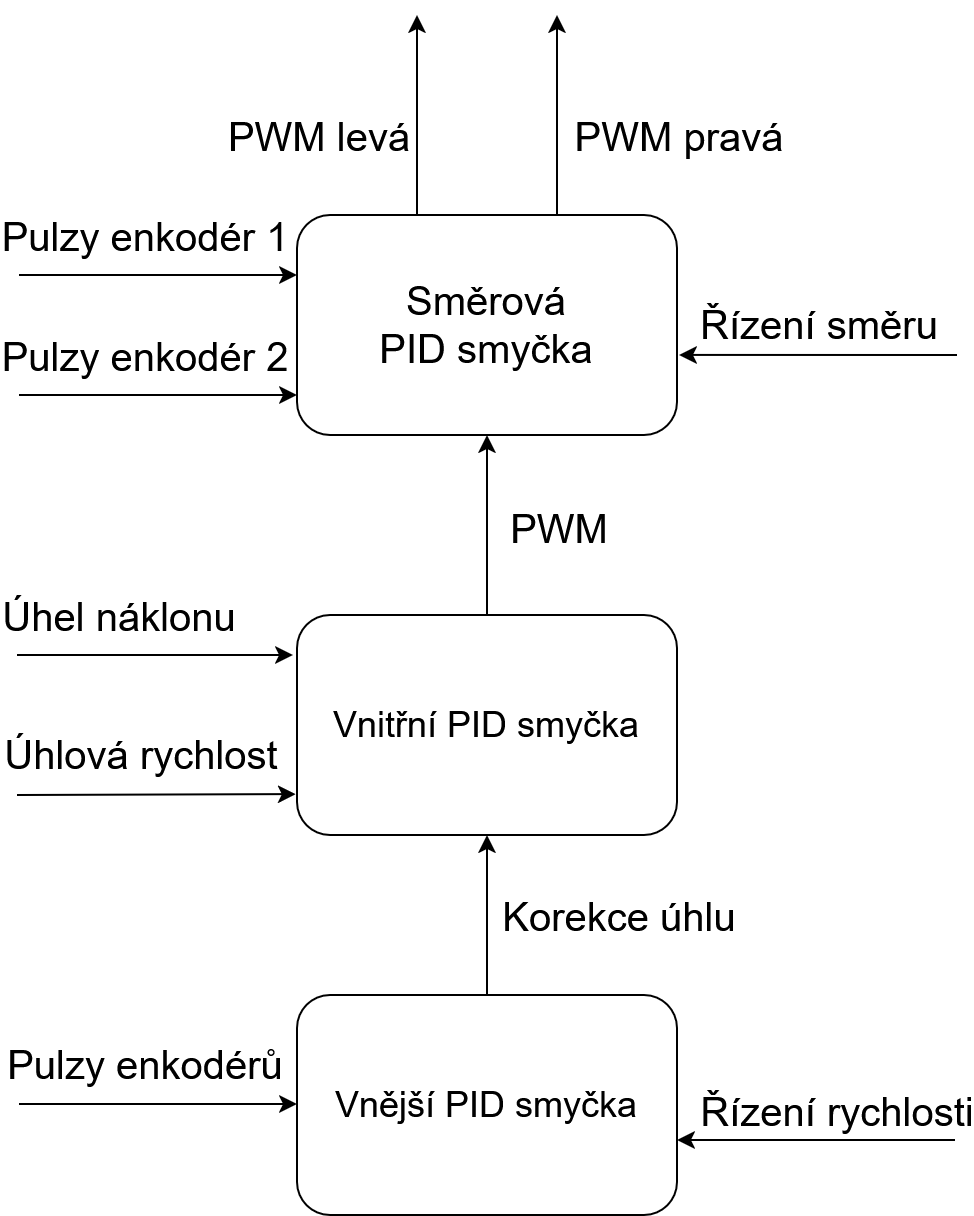
\includegraphics[width=0.75\linewidth]{obrazky-figures/PID.png}
    \caption {Diagram regulačních smyček, vytvořeno nástrojem https://app.diagrams.net}
    \label{PID}
\end{figure}

\subsection*{Vnitřní PID smyčka}
Vnitřní smyčka je navržena, aby podle vstupních dat stabilizovala robota ve vzpřímené poloze. Má dva vstupy: úhel náklonu (reprezentující deviaci od výchozího úhlu -- 0 stupňů) a úhlovou rychlost (reprezentující rychlost změnu úhlu náklonu). Výstupem vnitřní smyčky je hodnota PWM v rozsahu <-255; 255>, která určuje sílu a směr otáčení motorů. 

Chyba se vypočítává z úhlu náklonu -- jedná se o číslo opačné k naklonění. Do výpočtu chyby je navíc přidána kompenzace úhlu, která pochází z vnější PID smyčky. Výpočet chyby tedy vypadá takto:

\[
\text{chyba} = -(\text{úhel náklonu} + \text{kompenzace})
\]

V následujícím výčtu je uvedený postup výpočtu složek regulátoru:

\begin{enumerate}
  \item{\textbf{Proporcionální složka} poskytuje přímou reakci na chybu náklonu. Aby regulátor poskytoval dostatečně silnou reakci už při malé chybě, je k absolutní hodnotě chyby přičtena konstanta 0.5. Protože potřebná reakce motoru není s narůstající chybou náklonu lineární, je hodnota chyby (už zvýšená o dříve zmíněnou konstantu) umocněna číslem 1.1. Díky tomu proporcionální složka dokáže poskytnout silnou reakci při vysokém náklonu, ale zároveň citlivou reakci při náklonu malém.
  
\[
\text{proporcionální složka} = \left| \text{chyba} + 0.5 \right|^{1.13} \cdot \text{znaménko chyby}
\]
  
  }
  \item{\textbf{Integrační složka} akumuluje předchozí chyby náklonu, čímž potlačuje perzistentní chybu. Aby se zabránilo saturaci integrační složky (tzv. integral windup), sleduje regulátor úhlovou rychlost a integrační složku zvyšuje jen v případě, že chyba náklonu roste nebo je stálá. Pokud chyba klesá, je integrační složka při každém průchodu smyčkou násobena konstantou 0.98, což zabrání přehnané reakci regulátoru. Pokud úhel náklonu změní znaménko, je integrační složka násobená v každém dalším průchodu hodnotou 0.85, jinak by integrální složka nežádoucím způsobem ovlivňovala celkový výstup. 
  } 

\begin{align*}
&\text{if } \left( -\text{znaménko chyby} \cdot \text{úhlová rychlost} < 0 \;\text{\&\&}\; \left| \text{integrační složka} \right| > 1 \right) \\
&\quad \Rightarrow \text{integrační složka} = 0.98 \cdot \text{integrační složka} \\
&\text{else if } \left( \text{znaménko chyby} \cdot \text{integrační složka} < 0 \right) \\
&\quad \Rightarrow \text{integrační složka} = 0.85 \cdot \text{integrační složka} \\
&\text{else} \\
&\quad \Rightarrow \text{integrační složka} = \text{integrační složka} + \text{chyba} \cdot 10 ms
\end{align*}

  \item{\textbf{Derivační složka} nepoužívá (pro PID standardní) výpočet rychlosti změny z předchozích chyb, ale využívá k tomu přímo úhlovou rychlost. To je možné z důvodu, že úhlová rychlost je derivací úhlu náklonu. Tímto způsobem je získán čistší výsledek. Navíc má díky tomuto řešení derivační složka rychlejší reakci, než při výpočtu ze změn úhlu.}

 \[
 \text{derivační složka} = -\text{úhlová rychlost}
 \]
  
\end{enumerate}

\subsection*{Vnější PID smyčka}
Vnější PID smyčka koriguje výstup smyčky vnitřní. Na vstupu přijímá průměr z hodnot enkodérů 1 a 2 -- ten reprezentuje, jak daleko od výchozí pozice se robot odchýlil. Na základě intenzity vychýlení určuje regulátor korekci, kterou předává vnitřní smyčce.

Ve vnější PID smyčce má největší roli \textbf{derivační složka}. Ta je, podobně jako proporcionální složka ve vnitřní smyčce, umocněná číslem 1.13. Díky tomu při náhlé změně rychlosti pohybu (například postrčení robota) velmi rychle zvýší potřebnou korekci a nakloní robota v opačném směru, než je směr pohybu, čímž ho zabrzdí. Proporcionální a integrační složka slouží k návratu robota do původní pozice. 

Vnější smyčka také zajišťuje pohyb robota. Metoda \textbf{set\_speed} uměle navyšuje chybu. Na to smyčka reaguje náklonem na kýženou stranu a na to navázaným pohybem.

\subsection*{Směrová PID smyčka}
\label{turn}
Hlavním úkolem směrové smyčky je udržování směru. Každý motor má mírně odlišný statický odpor, takže při stejné PWM hodnotě se motory netočí stejně -- to platí hlavně při velmi nízkých hodnotách, kdy se motory teprve dávají do pohybu. Směrová PID smyčka má na vstupu hodnoty z obou enkodérů a počítá rozdíl mezi nimi. Vypočítává následně korekci. Korekce je na motory aplikována tímto způsobem:

\begin{align*}
\text{korekce} &= \text{směr(pulzy1, pulzy2)} \\
\text{PWM levá} &= \text{základní PWM} + \frac{\text{korekce}}{2} \\
\text{PWM pravá} &= \text{základní PWM} - \frac{\text{korekce}}{2}
\end{align*}

K manuálně ovládanému zatáčení robota má třída směrového regulátoru metodu \textbf{turn}. Ta uměle navyšuje chybu mezi stranami a regulátor reaguje navýšením rozdílu PWM mezi motory.

Metoda \textbf{turn\_deg} slouží k přesnému zatočení o zadaný počet stupňů. Pomocí následujícího výpočtu se určí, jakou chybu je potřeba nastavit pro každou stranu, aby se robot otočil o stanovený počet stupňů -- výsledek se tedy ještě musí vynásobit dvěma. V potaz se bere, že otáčení probíhá na místě, tedy kola se točí v opačném směru.


\begin{itemize}
  \item Rozlišení enkodéru (PPR): \( 734 \)
  \item Poloměr kola:  \( \text{r} = 67 \, \text{mm} \)
  \item Rozvor (vzdálenost mezi koly): \( L = 270 \, \text{mm} \)
  \item Cílový úhel otočení: \( \theta \, \text{(ve stupních)} \)
  \item Obvod kola: 
  \[
  o = 2\pi \cdot r = 2\pi \cdot 67 = 421 \text{mm}
  \]
\end{itemize}


\paragraph{1. Poloměr otočení:}
\[
R = \frac{L}{2} = \frac{270}{2} = 135 \, \text{mm}
\]

\paragraph{2. Délka oblouku, který kolo opíše:}
\[
s = 2\pi R \cdot \left( \frac{|\theta|}{360} \right) = 2\pi \cdot 135 \cdot \left( \frac{|\theta|}{360} \right)
\]

\paragraph{3. Potřebný počet otáček kola pro opsání oblouku o délce \( s \):}
\[
\text{rev} = \frac{s}{o} = \frac{2\pi \cdot 135 \cdot \left( \frac{|\theta|}{360} \right)}{421} = \frac{2\pi \cdot 135 \cdot |\theta|}{360 \cdot 421}
\]

\paragraph{4. Počet pulzů enkodérů:}
\[
\text{pulzy} = \text{rev} \cdot \text{PPR} = \left( \frac{2\pi \cdot 135 \cdot |\theta|}{360 \cdot 421} \right) \cdot 734
\]

\subsection*{Finální rovnice}
\[
\boxed{
\text{pulses} = \frac{1101\pi \cdot |\theta|}{842}
}
\]

\subsection*{Příklad: otočka o 90°}
\[
\text{pulses} = \frac{1101\pi \cdot 90}{842} \approx 370 \, \text{pulzů}
\]





\section{Dálkové ovládání}
\label{remote}
Dálkové ovládání probíhá pomocí aplikace Blue Dot \cite{bluedot}. Ta nabízí nastavitelné uživatelské prostředí bez nutnosti jakéhokoliv programování na straně telefonu -- vše se nastavuje přímo v kódu, v případě robota je to v ROS2 uzlu \textbf{bluetooth\_node}. Uživatelské rozhraní následně slouží jak k ovládání robota, tak ke zobrazení jeho stavu.

Výchozí obrazovka (obrázek \ref{bluedot} vlevo) ve vrchní části (čísla 1, 2, 3) zobrazuje stav senzorů (akcelerometr a gyroskop, enkodér, ultrazvukový senzor). ROS2 uzel obsluhující senzor (každý senzor má svůj vlastní uzel) posílá při inicializaci zprávu o připravenosti. Po obdržení zprávy příslušná kontrolka změní barvu z červené na zelenou. Tlačítko \textbf{č. 4} slouží k restartu programu. Po stisknutí spouští skript \textit{robot\_reset.sh}, který korektně ukončí celý ROS2 program a znovu ho spustí. To je vhodné využít ve chvíli, kdy jedna ze stavových kontrolek hlásí, že některý ze senzorů nebyl inicializován.

Tlačítko \textbf{č. 5} spouští balancování. O aktivním balancování informuje barva tlačítka, která se změní na zelenou. Pokud je balancování aktivováno a robot je vleže (úhel náklonu je větší než 45 stupňů), je aktivován zdvihací režim \ref{zdvih}. Tlačítko \textbf{č. 6} aktivuje autonomní jízdu (o stavu informuje barva tlačítka -- žlutá/zelená).

Poslední tlačítko \textbf{č. 7} přepíná režim ovládání na \textbf{joystick} (obrázek \ref{bluedot} vpravo). Ten umožňuje manuálně ovládanou jízdu pohybem prstu po kruhu -- pohyb vpřed/vzad, otáčení na místě, jízdu a zatáčení v jeden okamžik. Zpět na úvodní obrazovku se lze přepnout dvojím poklepáním na joystick.

\begin{figure}[H]
  \centering
  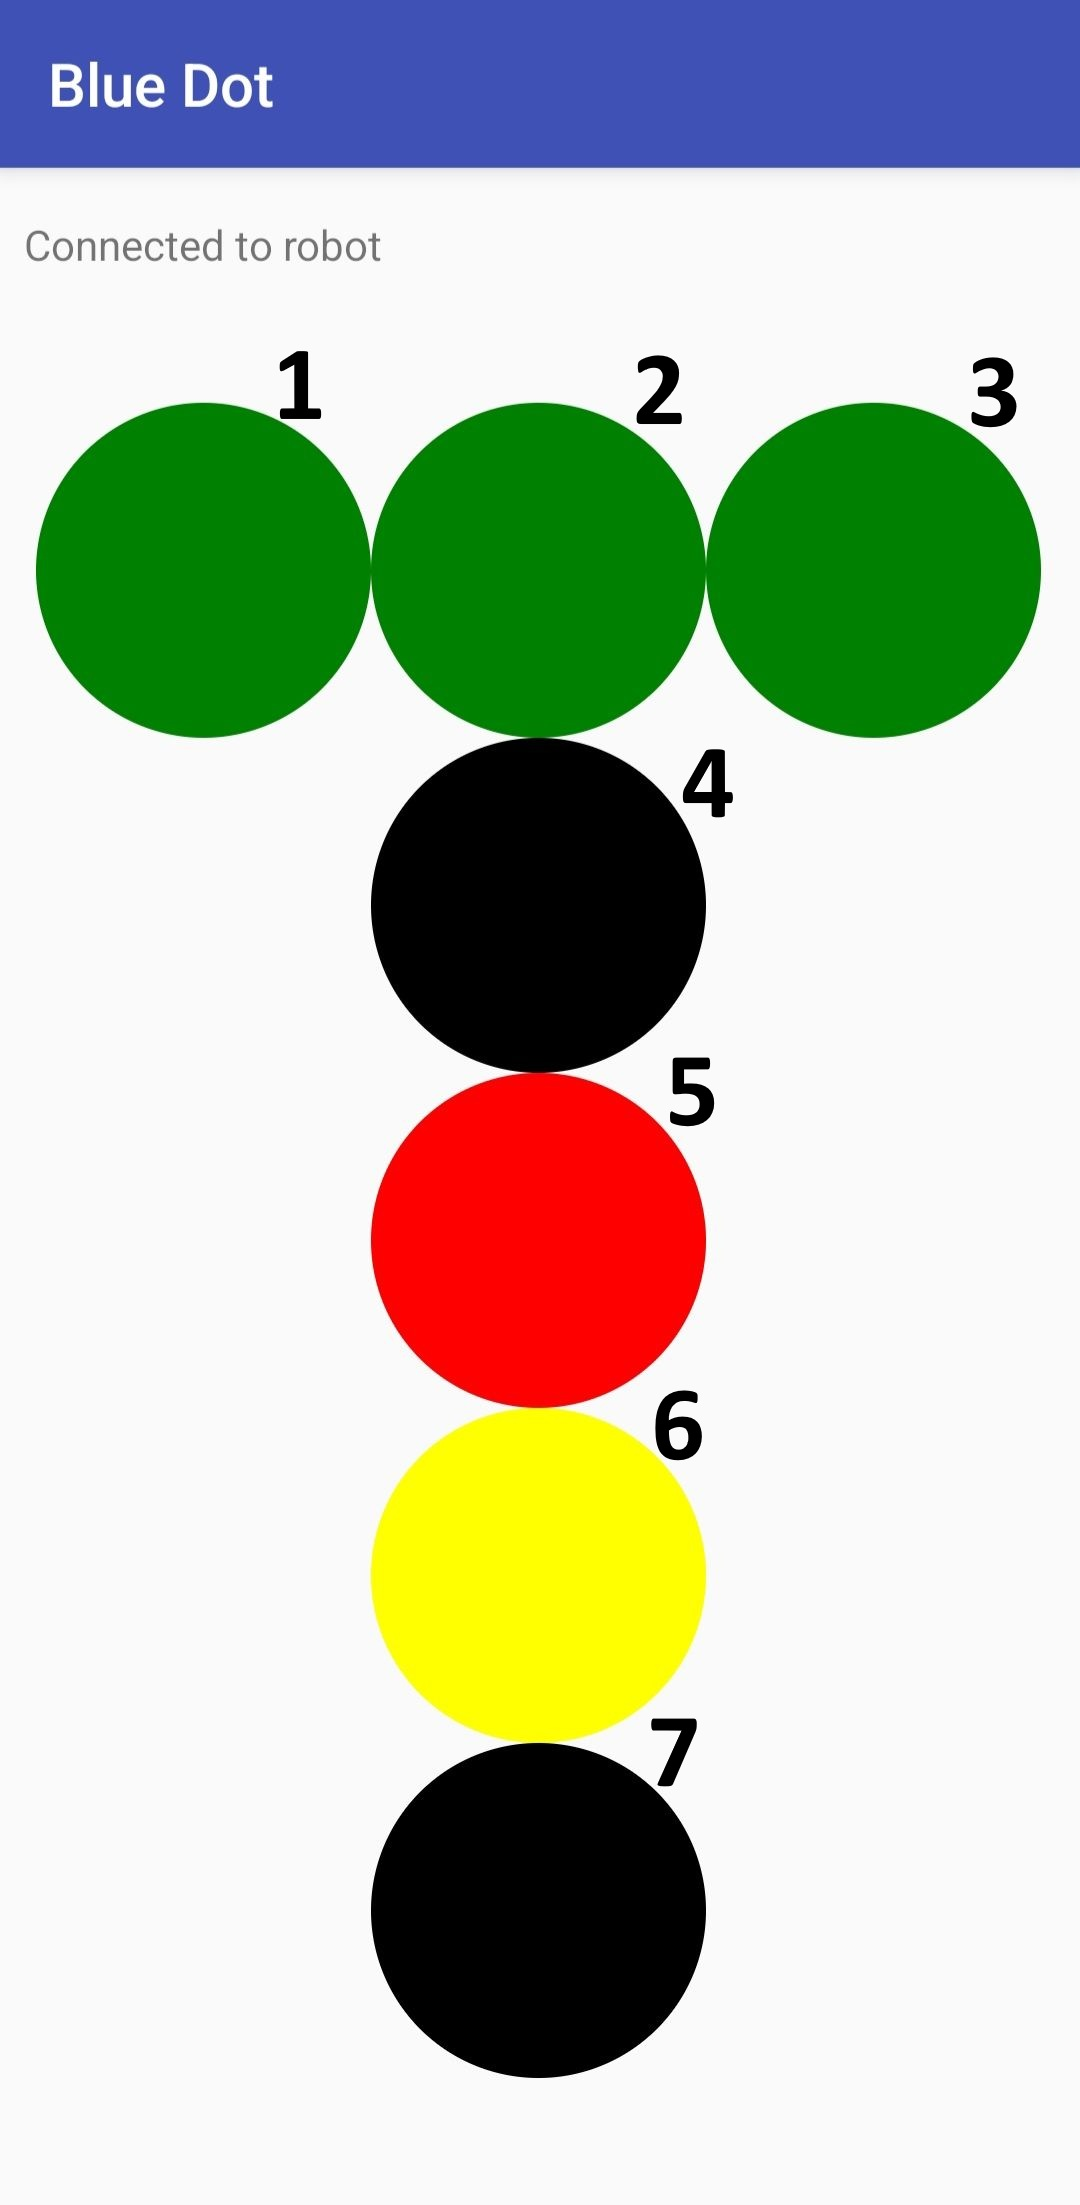
\includegraphics[width=0.48\linewidth]{obrazky-figures/buttons.jpg}%
  \hspace{1pt}\vrule width 1pt\hspace{1pt}%
  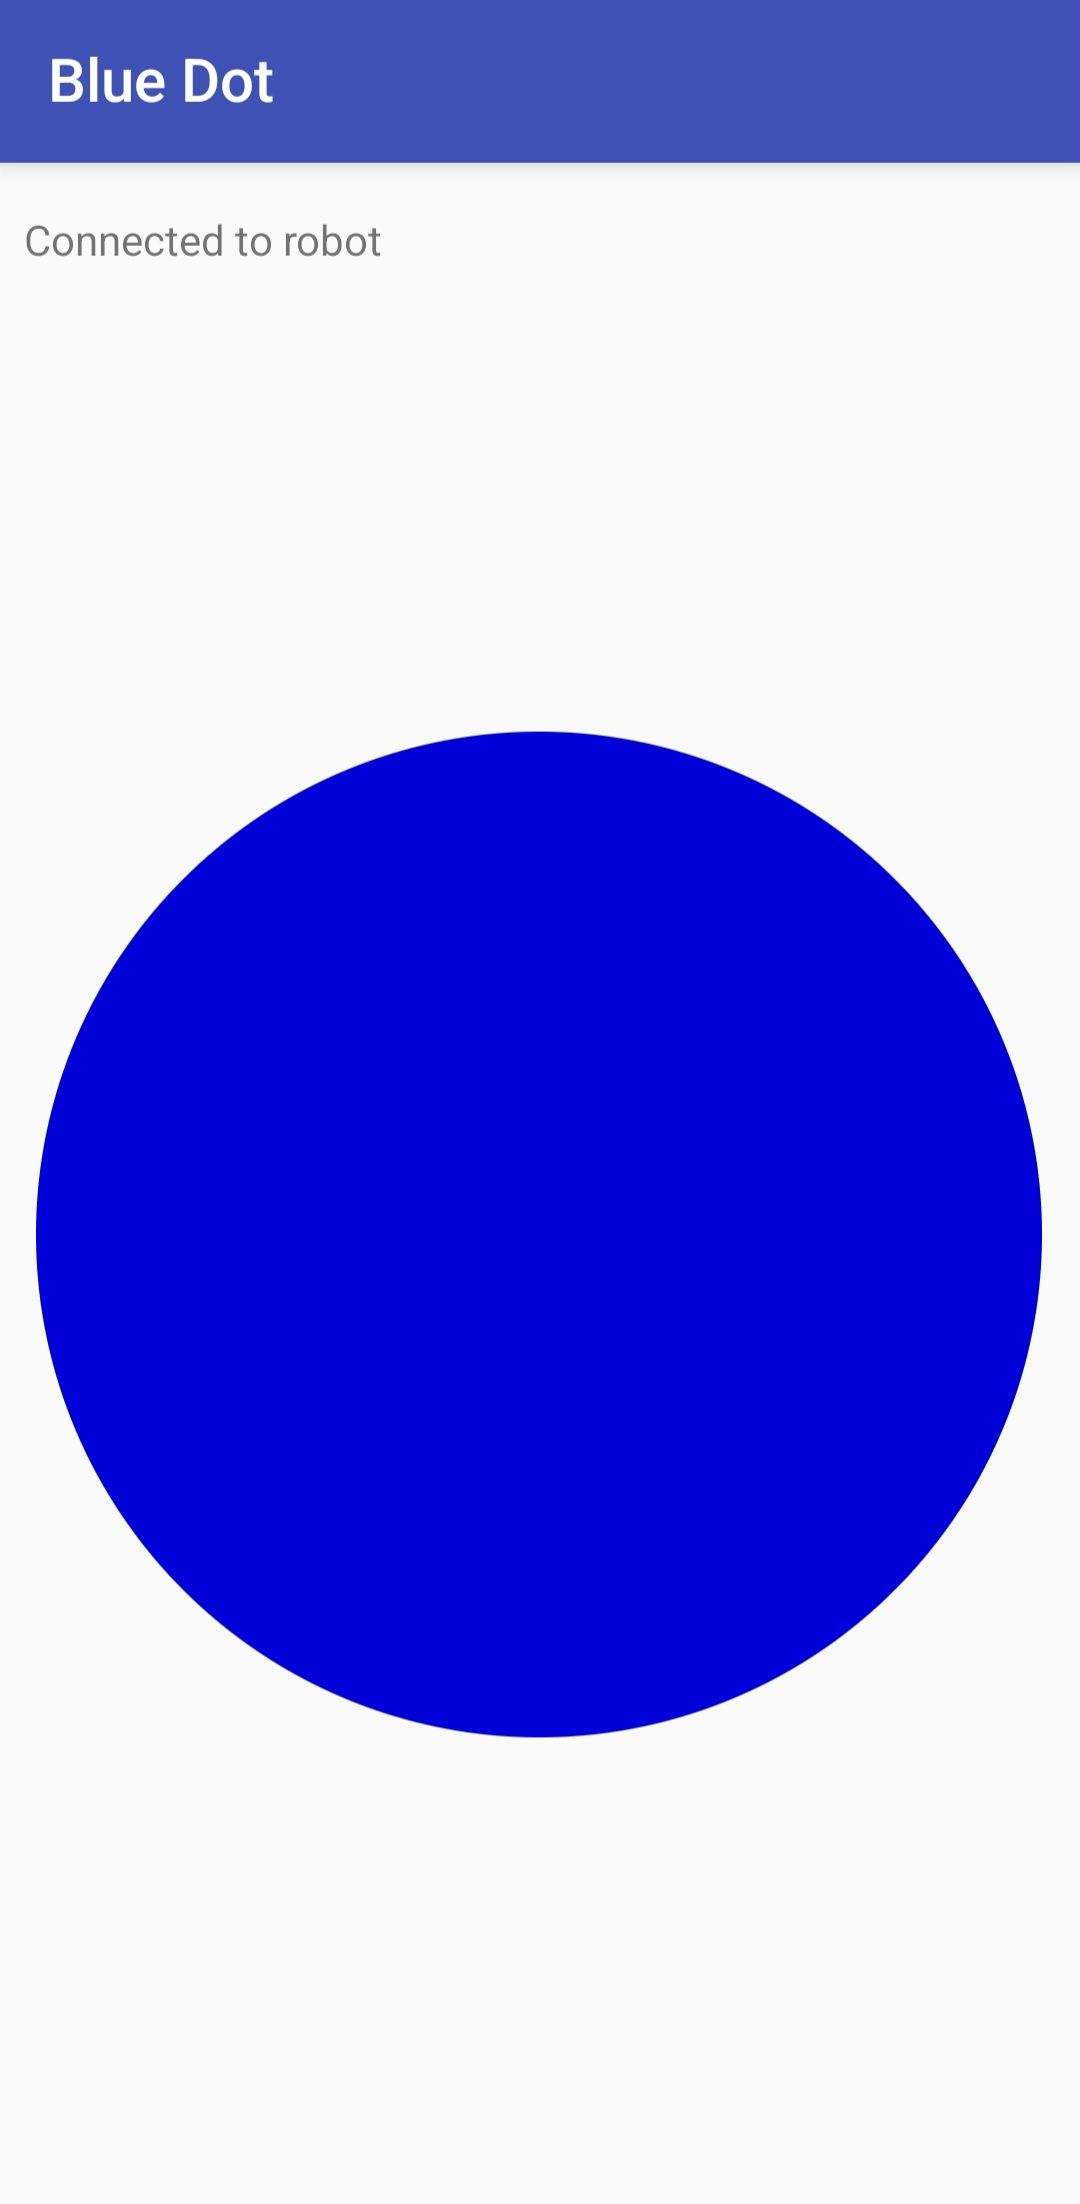
\includegraphics[width=0.48\linewidth]{obrazky-figures/joystick.jpg}
  \caption{\textbf{Legenda:} \textbf{1:} stav IMU, \textbf{2:} stav enkodéru, \textbf{3:} stav měřiče vzdálenosti, \textbf{4:} restart, \textbf{5:} zapnout balancování, \textbf{6:} autonomní režim, \textbf{7:} přepnout na joystick. \textbf{Vpravo:} joystick}
  \label{bluedot}
\end{figure}

\subsection*{Autonomní jízda}
Vedle režimu manuálního ovládání je robot schopný i jednoduché autonomní jízdy. Potom, co je autonomní jízda aktivována z mobilní aplikace, její řídící funkce dá robotovi povel k pohybu vpřed pomocí metody vnějšího PID regulátoru \textbf{set\_speed}. Pokud ultrazvukový senzor vzdálenosti nezaznamená žádnou překážku blíže než jeden metr, robot pokračuje stabilní rychlostí. Při zaznamenané překážce začne robot snižovat rychlost a při vzdálenosti od překážky 20 cm úplně zastaví. Následně pomocí metody směrového PID regulátoru \textbf{turn\_deg} provede otočku od 90° vpravo. Pokud po dokončení otáčení senzor snímá překážku blíže než 50 cm, provede robot otočku o 180°, aby na snímal opačnou stranu. Pokud je i na této straně překážka blíže než 50 cm, robot se otočí o 90° vpravo (tedy o 180° oproti výchozí pozici) a jede tímto směrem.

Algoritmus pohybu tedy vypadá následovně:

\begin{align*}
&\text{if } \left(\text{vzdálenost} > 100 \right) \\
&\quad \Rightarrow \text{set\_speed(10)} \\
&\text{else if } \left(\text{vzdálenost} < 100 \text{ \&\& } \text{vzdálenost} > 20\right) \\
&\quad \Rightarrow \text{set\_speed(scale(vzdálenost))} \\
&\text{else} \\
&\quad \Rightarrow \text{set\_speed(0)} \\
&\quad \Rightarrow \text{turn\_deg(90)} \\
&\quad \text{if } \left(\text{vzdálenost} < 50 \right) \\
&\qquad \Rightarrow \text{turn\_deg(180)} \\
&\qquad \text{if } \left(\text{vzdálenost} < 50 \right) \\
&\quad\qquad \Rightarrow \text{turn\_deg(90)} \\
\end{align*}

\section{Zdvih ze země}
\label{zdvih}
Robot má schopnost zdvihnout se ze země do vzpřímené polohy. Vzpřimovací režim (stand--up mode) je aktivován ve chvíli, kdy je v mobilní aplikaci zapnuto balancování a zároveň je úhel náklonu větší, než 60 stupňů. Na 35 iterací řídící smyčky (což je při frekvenci 100 Hz 350 ms) je obrácen směr otáčení motorů. Protože je v tu chvíli náklon robota přibližně 75 stupňů, vnitřní PID regulátor reaguje nastavením síly motorů na maximum. Robot se tedy dá do pohybu opačným směrem, než by byla obvyklá korekce při balancování. Během 350 ms pohybu získá robot dostatečnou hybnost, takže když se motory začnou točit opačným směrem, robot je „vystřelen“ do vzpřímené pozice. V tu chvíli už balanční mechanismus zajistí, že robot zůstane ve vzpřímené poloze. 

\chapter{Testování a vyhodnocení}
\label{chap6}
V následující kapitole je popsán průběh testování, jeho výsledky a popis problémů, na které se narazilo. Pokud není řečeno jinak, jsou výsledky na grafech zaznamenány při plném stavu baterie (12,6 V)

\section{První pokusy}
Balancování robota bylo nejprve řešené pouze vnitřním PID regulátorem, který reaguje na úhel náklonu a úhlovou rychlost. Projevila se zde ovšem nevhodná volba motorů, která to znemožňovala. Použitý model motoru má velkou mrtvou zónu -- ta zabírá spodní část PWM rozsahu. Je způsobena zvoleným typem motorů. Stejnosměrné kartáčované motory vybavené převodovkou mají totiž vysoký statický odpor. V praxi to lze vidět na grafu \ref{deadzone}. Červenou barvou je znázorněn sílící signál PWM a modrou barvou počet výstupních pulzů enkodéru. Hodnota pulzů začíná růst až při hodnotě PWM 31, což znamená, že mrtvá zóna tvoří 12,2 \% rozsahu PWM.

Kvůli tomuto problému je minimální rychlost otáčení přibližně 7 RPM. Regulátor tedy nemohl korigovat malé chyby do přibližně 1,5 stupně náklonu. Snaha o korekci tak malého úhlu totiž kvůli vysoké minimální rychlosti vedla k přestřelení na opačnou stranu a způsobila rychlou oscilaci. Amplituda oscilací se stále zvyšovala, dokud se robot nedostal do náklonu ze kterého se již nedokázal dostat zpět a spadl. Situace je znázorněna na grafu \ref{inner} Při pokusech o předcházení oscilacím snížením PID koeficientů se robot dostával do nenapravitelného náklonu okamžitě.

\begin{figure}[H]
  \centering
  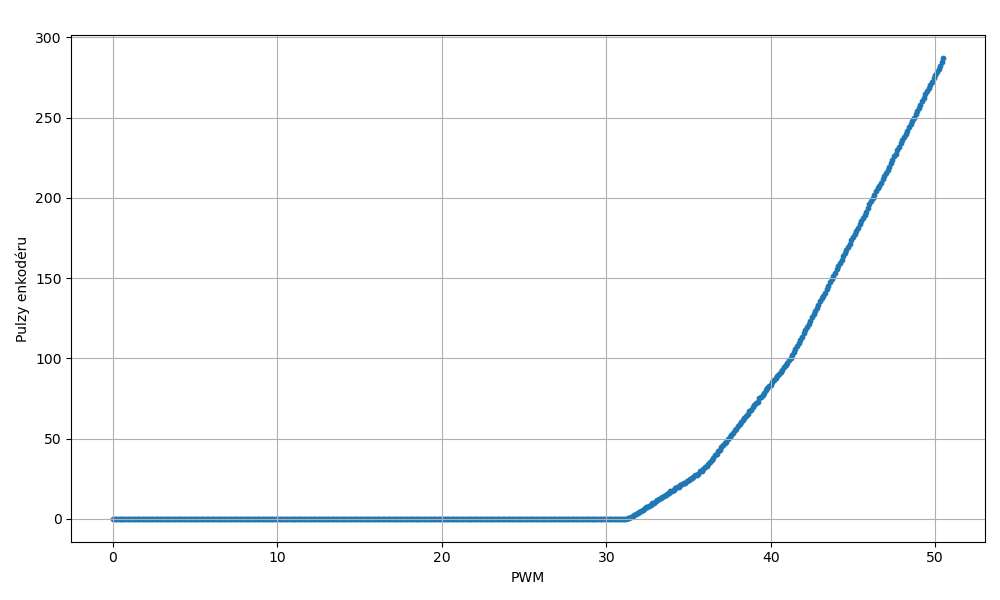
\includegraphics[width=1.\linewidth]{obrazky-figures/deadzone.png}%
  \caption{Graf znázorňuje při jaké hodnotě signálu PWM se začínají točit motory.}
  \label{deadzone}
\end{figure}

\begin{figure}[H]
  \centering
  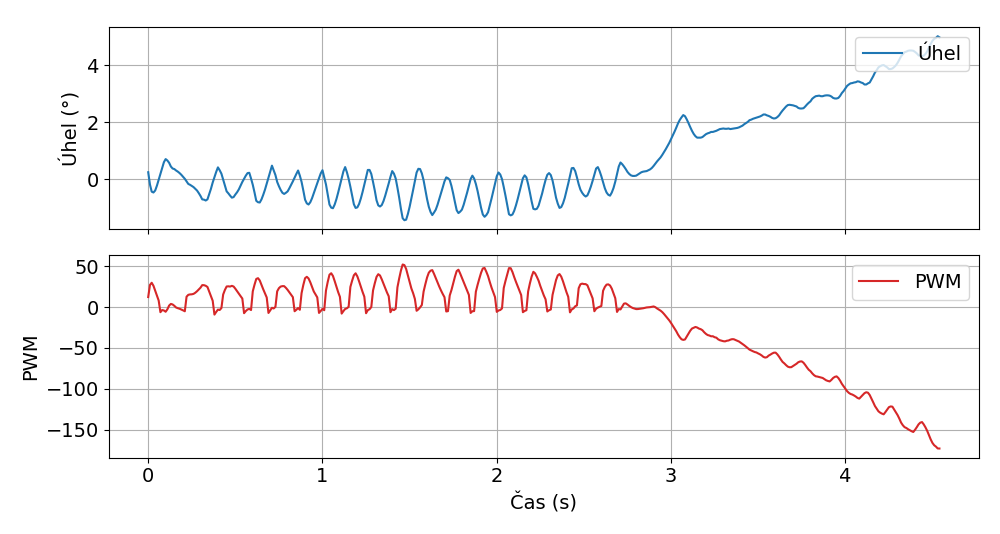
\includegraphics[width=1.\linewidth]{obrazky-figures/inner.png}%
  \caption{Graf znázorňuje průběh balancování bez vnějšího PID regulátoru.}
  \label{inner}
\end{figure}

\section{Kombinace vnějšího a vnitřního regulátoru}
Doplnění vnějšího PID regulátoru, který posílá korekci úhlu do vnitřního regulátoru, umožnilo robotu balancovat. Díky založení regulátoru na výstupu z enkodérů je možné snížit PID koeficienty vnitřního regulátoru bez rizika, že robot sám spadne do náklonu, který nedokáže korigovat. Tím se předejde oscilacím, které byly způsobeny příliš silnými PID koeficienty.

Kvůli problému s nevhodně zvolenými motory, který byl probrán v předchozí sekci, robot nedosahuje dokonale plynulého balancování ani s vnějším regulátorem. Znázorněno je to na grafu \ref{normal} -- je zde vidět, že robot pomalu osciluje mezi stranami s periodou cca 2,5 sekundy. Oscilace je ale stabilní a ani po delším čase stání na místě nemá tendenci zvyšovat svou intenzitu.

Díky použití PID regulátoru je robot schopný pokračovat v balancování i při malé změně těžiště. V experimentu znázorněném na grafu \ref{load} bylo na vrchní stranu robota umístěno železné závaží o hmotnosti 1,1 kg. Na balancování se to projevilo hladším chodem, ale zároveň i většími výkyvy do stran (zároveň je potřeba silnější PWM signál). Hladší chod se zde objevuje z důvodu, že vyšší hmotnost se přirozeně chová jako tlumič vibrací. A protože vzhledem k problému s příliš vysokou minimální rychlostí otáčení motorů, který je zmíněn v předchozí sekci, robot za normálních okolností reaguje na korekce rychlou změnou náklonu -- přidání závaží tuto reakci zmírní.

\begin{figure}[H]
  \centering
  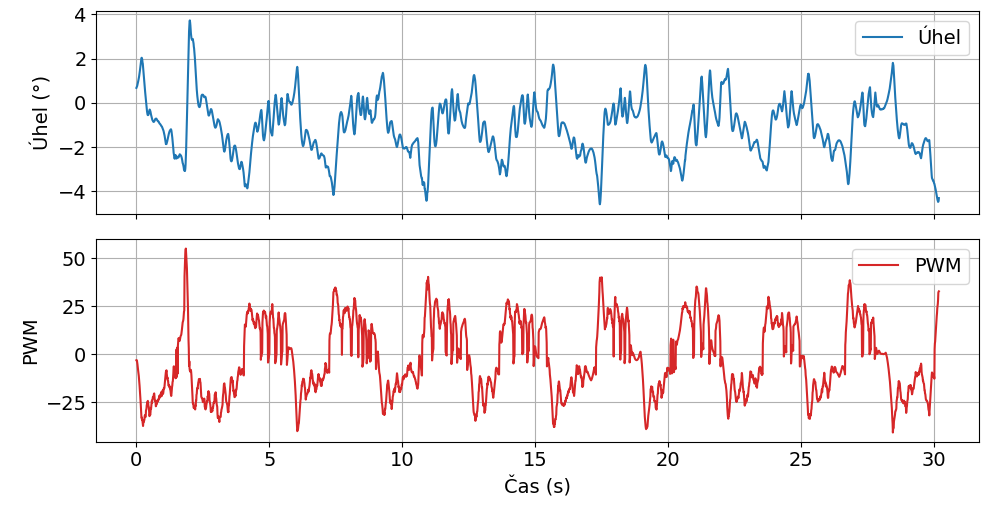
\includegraphics[width=1.0\linewidth]{obrazky-figures/normal.png}%
  \caption{Balancování na místě s kombinací vnějšího a vnitřního regulátoru.}
  \label{normal}
\end{figure}

Robot je schopný reagovat i na postrčení a snahu o jeho vychýlení z rovnováhy. Taková situace je zaznamenaná na grafu \ref{push}. Přibližně v čase 4.7 sekundy nastává situace, kdy je robot postrčen (prudké zvýšení úhlu náklonu nad 5 stupňů). Na akci okamžitě reaguje regulátor a PWM signál dosáhne hodnoty přes 200. Robot se při postrčení dostal do vyšší rychlosti a zároveň se vychýlil od výchozí pozice -- na to reaguje vnější regulátor, který nastaví vysokou korekci. Robot se nakloní až téměř 10 stupňů na stranu opačnou té, do které jede. Situace je vidět na grafu v čase 6 sekund. Do normálního stavu se robot vrací asi 4 sekundy po události.

\begin{figure}[H]
  \centering
  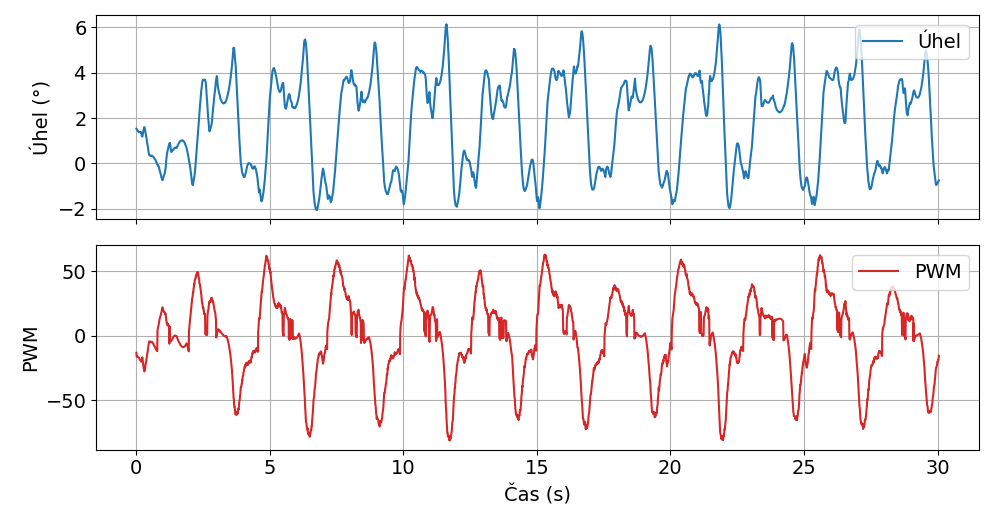
\includegraphics[width=1.0\linewidth]{obrazky-figures/load1.png}%
  \caption{Balancování na místě se zátěží}
  \label{load}
\end{figure}

\begin{figure}[H]
  \centering
  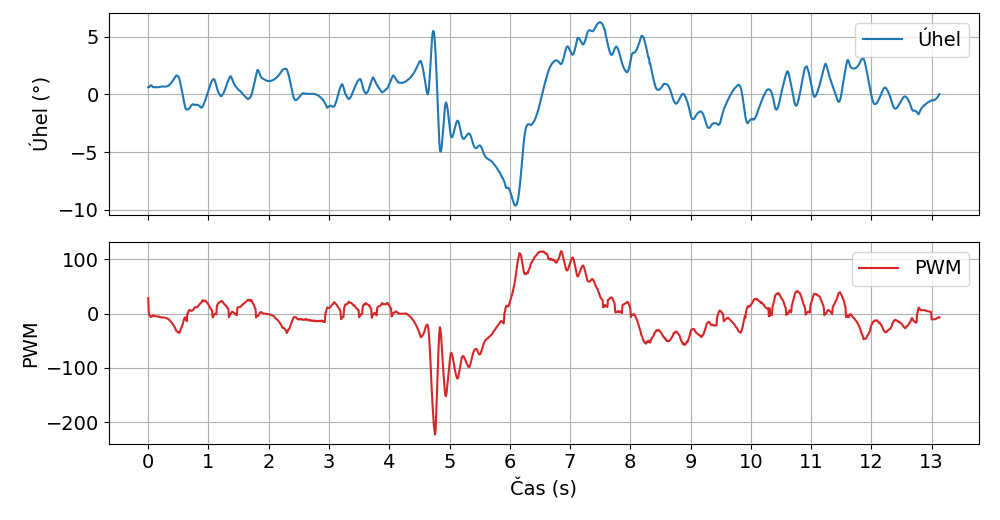
\includegraphics[width=1.0\linewidth]{obrazky-figures/push.png}%
  \caption{Reakce robota na postrčení do strany.}
  \label{push}
\end{figure}

V dalším experimentu byla vyzkoušena schopnost robota dostat se z velkého vychýlení do vzpřímené polohy bez použití \textbf{zdvihací sekvence} (tedy bez opačného chodu motorů, který pomůže vzpřímení).

Robot byl manuálně držen v úhlu náklonu asi 30 stupňů a v mobilní aplikaci bylo aktivováno balancování. Následovala okamžitá korekce, kdy v signál PWM v počáteční fázi dosáhl maximální hodnoty 255. K úplné korekci náklonu došlo za méně než jednu vteřinu. Situace je zaznamenána na obrázku \ref{off}.

\begin{figure}[H]
  \centering
  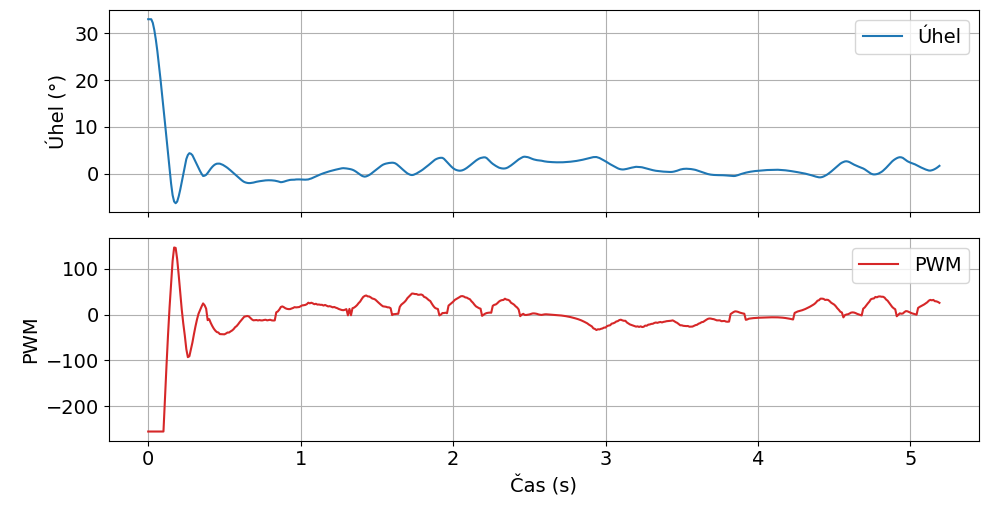
\includegraphics[width=1.0\linewidth]{obrazky-figures/off.png}%
  \caption{Aktivace stabilizace v náklonu.}
  \label{off}
\end{figure}

\subsection*{Změna chování při poklesu napětí baterie}
Úroveň napětí baterie ovlivňuje, s jakou silou se otáčí motor při dané hodnotě PWM. Při napětí baterie 11 V a PWM 100 motor nevyvine takový kroutící moment, jako by vyvinul při stejné hodnotě PWM a napětí 12 V.

Při experimentu bylo vyzkoušeno balancování při hodnotě nabití baterie 10,1 V. Na obrázku \ref{low} lze vidět, chování robota se oproti stavu s nabitou baterií \ref{normal} příliš nezměnil.

\subsection*{Zdvih}
Zdvihnutí ze země je možné díky silným motorům a kvalitním kolům. Za ideálních podmínek (dřevěná podlaha, čistá kola) se robot dokáže vzpřímit za méně než jednu sekundu a bez dalších oscilací. Na obrázku \ref{stand-up} vidíme obrácený směr točení motorů (princip zdvihu je podrobně popsán v sekci \ref{zdvih}). V momentu, kdy se změní směr otáčení se začíná úhel náklonu přibližovat nule. Následuje malé přestřelení úhlu, které je ale okamžitě korigováno.

Byl proveden experiment, kdy byla kola robota úmyslně znečištěna tak, aby se snížila přilnavost. To sice při startu vedlo k vyššímu prokluzu, zdvihnutí ze země tím ale ohroženo nebylo.

\begin{figure}[H]
  \centering
  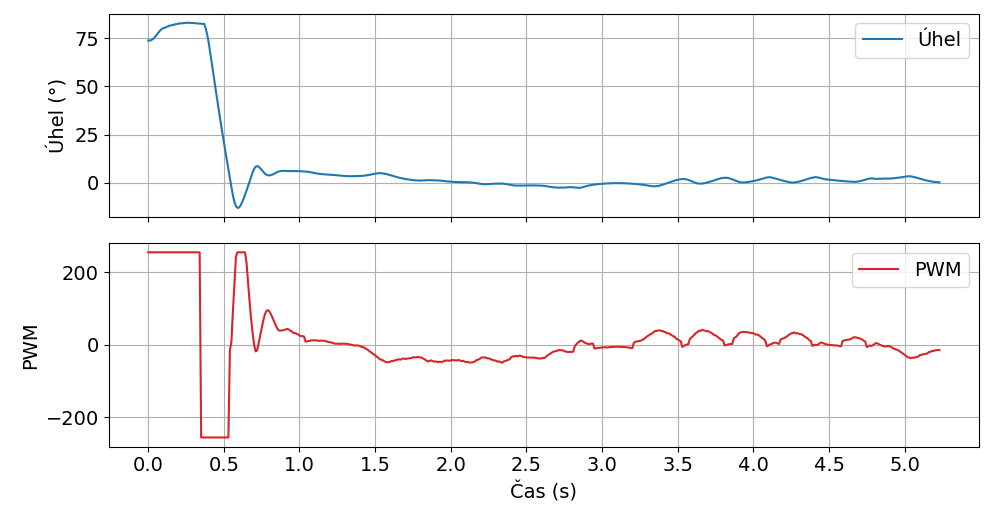
\includegraphics[width=1.\linewidth]{obrazky-figures/stand_up.png}%
  \caption{Zdvih robota.}
  \label{stand-up}
\end{figure}

\begin{figure}[H]
  \centering
  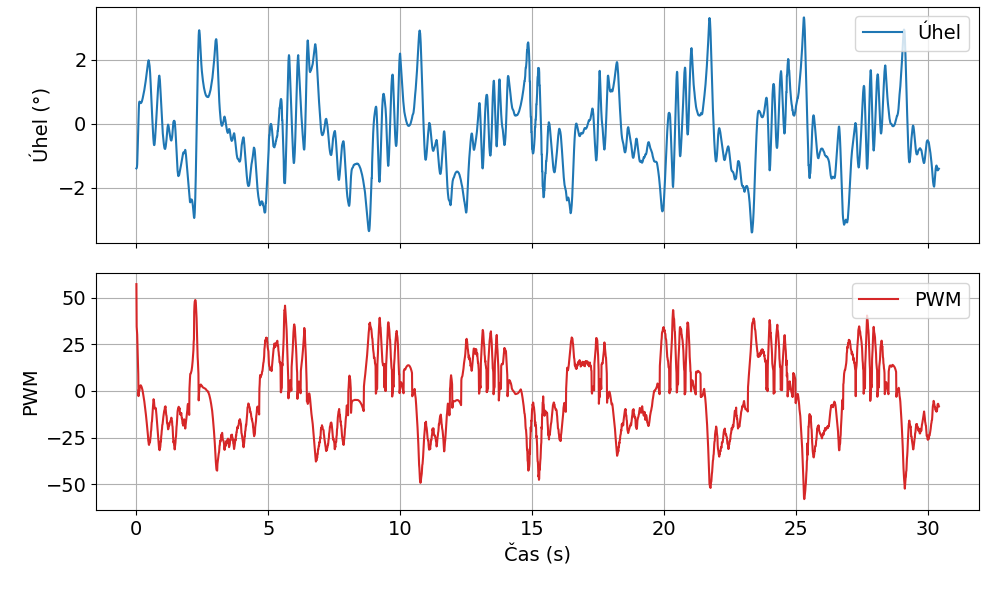
\includegraphics[width=1.0\linewidth]{obrazky-figures/low.png}%
  \caption{Balancování s baterií nabitou na 10,1 V.}
  \label{low}
\end{figure}

\section{Dálkové ovládání}
Dálkové ovládání pomocí joysticku v mobilní aplikaci je plně funkční. Robot se dokáže rychle pohybovat do všech stran, zatáčet v průběhu jízdy a provést otočku na místě.

\begin{figure}[H]
  \centering
  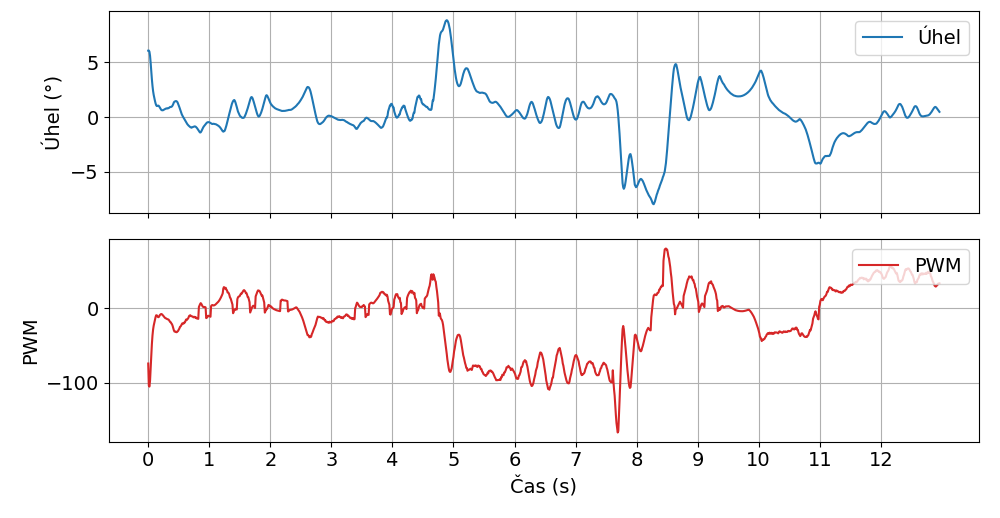
\includegraphics[width=1.0\linewidth]{obrazky-figures/move.png}%
  \caption{Robot v pohybu.}
  \label{move}
\end{figure}

Pohyb robota je ukázán na grafu \ref{move}. Začíná přibližně v čase 4,6 sekundy -- v tu chvíli je pomocí dálkového ovládání nastaven pohyb vpřed. V první chvíli robot reaguje zvýšením náklonu na stranu pohybu, ale po chvíli se náklon srovná. Ačkoliv při pohybu zůstává robot ve vzpřímené poloze s minimálním náklonem, pohyb lze vidět na průběhu hodnoty PWM, která při jízdě dosahuje síly signálu přibližně 100.

V čase 7,7 sekund ukončuje dálkové ovládání pohyb vpřed. Systém na to okamžitě reaguje změnou náklonu do směru opačného pohybu robota a prudkým zvýšením PWM, což vede k zastavení pohybu.
\begin{figure}[H]
  \centering
  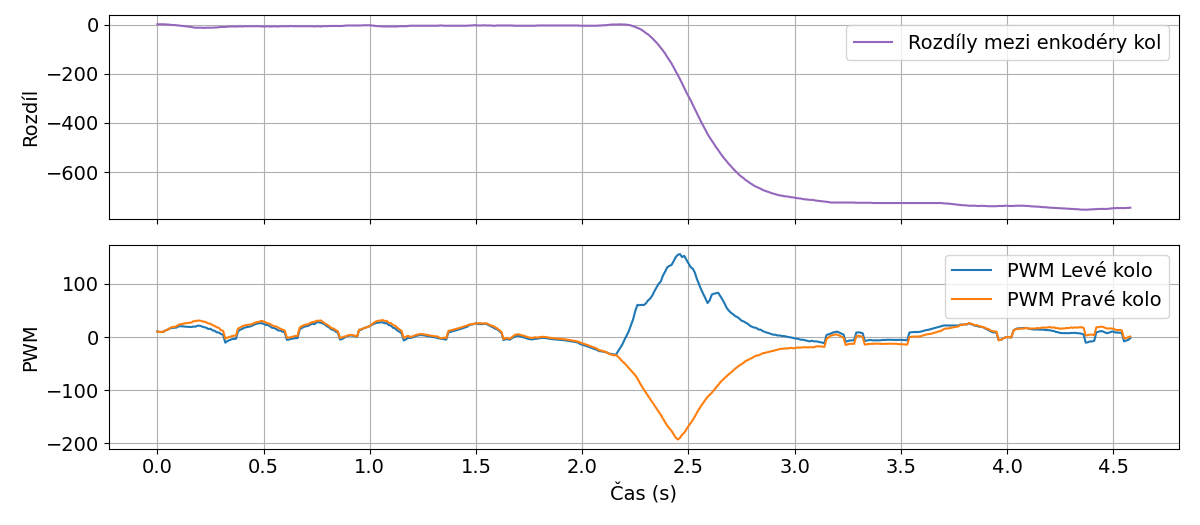
\includegraphics[width=1.0\linewidth]{obrazky-figures/turn.png}%
  \caption{Otočení o 90 stupňů na místě.}
  \label{turn_g}
\end{figure}

Přesné otočení o zadaný počet stupňů je na grafu \ref{turn_g}. Systém dostává příkaz na otočení od 90 stupňů na místě. Pomocí vzorce, který je odvozený v sekci \ref{turn} je vypočítáno, že každé kolo se musí otočit o 370 pulzů enkodéru opačným směrem -- tedy má vzniknout chyba 740 pulzů. Z průběhu grafu lze pozorovat, jakým způsobem je zatáčení implementováno. Směrový PID regulátor z požadovaného úhlu vypočítá hodnotu, kterou k jednomu z PWM signálů přičte a od druhého odečte. 

Podle vlastního měření pomocí úhloměru se robot otočil přesně o 91 stupňů. Chyba jednoho stupně může být způsobena prokluzem kol, nebo chybou měření enkodéru.

\section{Autonomní jízda}
Při autonomní jízdě se projevil málo kvalitní použitý měřič vzdálenosti. Ultrazvukový senzor hc-sr04 má problém registrovat objekty, které nemají pevný a hladký povrch. Problémem jsou i objekty, které nejsou proti senzoru kolmo, ale pod úhlem. Při větším náklonu robota může senzor chybně reagovat i na podložku, po které se robot pohybuje.

Výsledkem je, že robot při autonomní jízdě reaguje na falešná měření, případně na překážku reaguje pozdě a narazí do ní.


\chapter{Závěr}
\label{chap7}

Cílem této bakalářské práce bylo nastudování problematiky balancujících dvoukolových robotů a následné navrhnutí, sestavení a naprogramování takového robota. Důležitým aspektem projektu bylo použití řídící platformy Raspberry Pi bez jakýchkoliv pomocných kontrolérů.

Ač použití Raspberry způsobilo určité komplikace, ukázalo se toto řešení jako proveditelné. Pro správné fungování bylo ovšem nutné korektní nastavení operačního systému a dostatečné filtrování dat.

ROS2 se ukázalo být ideálním prostředím pro implementaci projektu takového typu a rozsahu. Umožňuje vysokou modularitu, a je proto snadné přidat třeba další senzor, pro který stačí vytvořit nový ROS2 uzel komunikující se zbytkem projektu.

Ve finále bylo dosaženo funkčního balancování za použití tří PID regulátorů. Robot se dokáže zdvihnout ze země a dokáže korigovat i velké náklony, které mohou vzniknout například postrčením. Dokáže si poradit i se změnou těžiště. Režim dálkového ovládání přes joystick v aplikaci funguje správně.

Práce by mohla být rozšířena použitím kvalitnějšího snímače okolí. V potaz by připadal LIDAR senzor, který by umožnil sestavit si mapu okolí. Autonomní mód by v tom případě mohl mít větší význam, než jen jednoduché vyhýbání se překážkám.

%===============================================================================

% Pro kompilaci po částech (viz projekt.tex) nutno odkomentovat
%\end{document}
